% Page 067 — page imprimée 64
% Carte : « Meyrueis et ses trois vallées »
% La carte est reproduite comme dans l'original, en orientation paysage.

\sectiondate{Meyrueis et ses trois vallées}{}

\begin{center}
    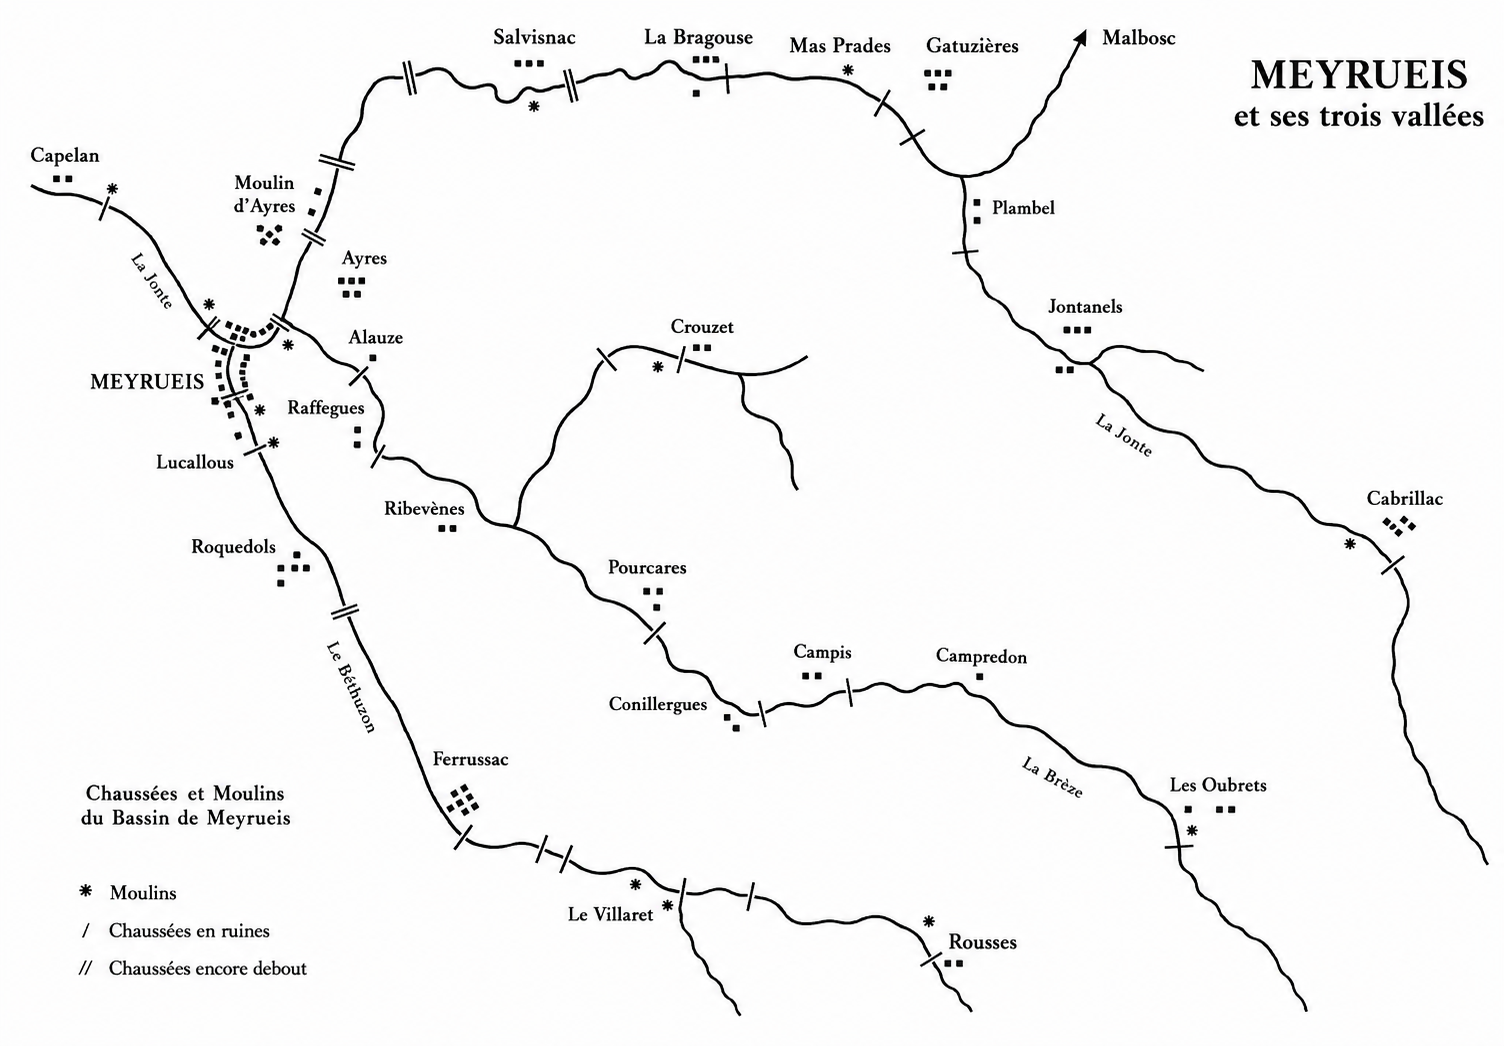
\includegraphics[angle=90,origin=c,width=\textwidth,height=0.9\textheight,keepaspectratio]{imgs/067.png}
\end{center}

% Page 068 — page imprimée 64 bis
% La vallée de la Jonte

\begin{center}
\fbox{\parbox{0.65\textwidth}{
\textbf{Meyrueis se trouve au confluent de trois vallées,\\
Jonte, Brèze et Béthuzon. Sans doute faut-il chercher\\
dans cette situation l’étymologie de son nom\\
« au milieu des rivières ».
}}}
\end{center}

\vspace{1em}

\textbf{Je vous propose de les remonter, l’une après l’autre.}

\vspace{1.5em}

\subsection{La vallée de la Jonte}


\medskip

C’est au pied du signal des Fons, au bas de la pelouse de l’Aigoual, près de la grande congère
qu’elle prend sa source. Ruisselet ruisseau, rivière elle cascade dans les gorges étroites des
Escarabits avant de baigner les maisons de Jontanels et de s’épanouir du côté de Gatuzières
abandonnant le granite et les schistes de sa naissance pour serpenter sous les hautes couronnes
calcaires du Méjean.

\medskip

Après Meyrueis elle sépare désormais Causse Noir et Causse Méjean ; les gorges deviennent
profondes abritant bien des grottes, celles de la Chèvre, de la Vigne et de Nabrigas, arcade des
bergers et, si bien cachée, la grotte Amélineau aux mille stalactites fistuleuses éblouissantes,
la perte des Hérans et la résurgence des Douze, le Roc Saint Gervais, et l’ermitage Saint
Michel avant de s’abandonner dans les eaux vertes du Tarn pour gagner l’Océan.

\medskip

Maintenant tel un pêcheur de truites, au grand dam des géographes, nous remontons son cours.
Barrée de nombreuses chaussées, la Jonte arrosait prés et jardins et faisait tourner de
nombreux moulins. L’un des plus anciens, le moulin de Capelan fut équipé postérieurement
d’une petite turbine qui permit l’électrification du village dans les années 1900, le moulin de
Malbois rue des Apiès, au centre du village, un des derniers à faire de la farine avec celui de
Gatuzières jusqu’en 1950-1960 environ. (22 moulins sur nos trois rivières vers 1850 !!!).

\medskip

Sur la rive gauche de la Jonte, à notre droite donc, après « l’arbre du poivre » (voir dans « La vallée
de la Brèze ») et la piscine se découpent les maisons d’Ayres et invisible, sous de grands arbres
entourés d’un haut mur se cache le Château d’Ayres dont nous connaissons l’histoire récente.

\medskip

Son moulin, le Moulin d’Ayres que l’on rejoint, à pied, par le Pont de Six Liards a connu bien
des évolutions, résumées dans les pages suivantes.

\medskip

Nous le quitterons pour remonter au plus près le cours de cet affluent du Tarn.

\medskip

Enfin tout près de la source de la Jonte, l’histoire de Cabrillac a été relatée par Yves Grellier
en 1991 « Cabrillac : Un hameau sur L’Aigoual ».

% Page 069 — page imprimée 65
% La famille Roussel du Villaret au Château d'Ayres

\subsubsection{La famille Roussel -- du Villaret au Château d’Ayres}


\medskip

\textbf{Il était une fois à Ayres}, hameau dominant la vallée de la Jonte, non loin de Meyrueis, un
château. Bien moins imposant mais plus ensoleillé et accueillant que celui de Roquedols, il
avait été construit au 7° siècle. Après bien des vicissitudes, une communauté monastique s’y
installe en 1025 puis l’abandonne au début du 16° siècle. Le château est acheté alors par une
famille protestante de Montpellier, les « de Galtier de Montauran », qui le fortifient.
Christophe de Galtier, chef de guerre énergique et violent, dirigera au nom du roi de Navarre,
la prise et le sac de La Canourgue en 1591 au cours duquel l’église fut incendiée.

\medskip

Lors de la guerre des camisards, en 1702, la troupe de Castanet suivi de la Rose, son fidèle
compagnon, vint camper au Château d’Ayres. \textit{« On fit une assemblée, relate Philippe
Chambon dans « Itinéraires Protestants en Languedoc », présidée par Castanet où se
rendirent les habitants de la cité, mais aussi, des soldats de la garnison, des officiers et même
des prêtres. A l’issue de ce culte une vingtaine de protestants de Meyrueis furent arrêtés.
Réaction immédiate des Camisards qui capturent une quinzaine de soldats et des officiers du
régiment de Cordes. Après négociation chacun relâcha ses otages et l’affaire se conclut par un souper, au château
d’Ayres, réunissant les chefs révoltés et le major du régiment qui assura n’avoir procédé aux
arrestations qu’à l’instigation des prêtres, qui prétendaient que la trêve signée par Cavaler et
Villars ne concernait pas les autres camisards. »}

\medskip

Plus tard le sénéchal d’Anduze, sur les ordres de Richelieu, démantela les deux tours ainsi que
les remparts du château et finalement après la Révocation de l’Edit de Nantes en 1685, Galtier
de Montauran fit amende honorable, abandonna le protestantisme pour sauver ses biens : le
château et son moulin, le moulin d’Ayres, ainsi que de nombreuses terres.
Mal lui en prit car les camisards l’incendièrent. Ses descendants « dilapidèrent l’héritage ».

\medskip

Déjà en 1736 Jean de Galtier de Montauran avait cédé le moulin du Château (Le Moulin
d’Ayres) à son meunier, \textit{« baillé à titre de loyer perpétuel et emphytéose, à Jean Rozier
originaire du Moulin d’Aumières ».}

\medskip

Mais c’est surtout le dernier Charles de Galtier de Montauran qui, joueur invétéré, fut dans
l’obligation de vendre, par morceaux successifs, une bonne partie des terres du château afin
de payer ses dettes de jeux.

\medskip

C’est ainsi qu’en janvier 1839, il doit régler 3000F au sieur Auradou, boulanger, 3.000F aussi
au sieur Agulhon et enfin 900F à un certain Jean Ribes. C’étaient de grosses sommes. Enfin le
château avec le bosquet est vendu au 19° siècle à une famille Nogaret qui voulait le
réhabiliter mais se décide assez rapidement à le revendre. Deux de leurs enfants reposent au
cimetière de Meyrueis.

% Page 070 — page imprimée 66
% La famille Roussel du Villaret au Château d’Ayres (suite)

\textbf{Il était une fois au Villaret}, hameau de la vallée du Béthuzon à sept km de Meyrueis une
famille de paysans, les Roussel qui possédaient une petite maison avec une grange attenante
actuellement rénovée par les Danjean-Henry. La vie était très dure mais on économisait sou
à sou et arriva le moment où la famille envisagea de descendre « à la ville » pour avoir une
vie plus facile. La ville c’était Meyrueis, bien sûr !

\medskip

Comment purent-ils acheter un café au bord de leur rivière, le Béthuzon ? Et à quelle époque ?
L’histoire ne le dit pas. Mais Antoine Roussel avait épousé une Valès, qui avait quelques
biens, sœur d’un certain Henry Valès, né à Meyrueis qui fit de très brillantes études de
Théologie à Montauban, d’où il sortit « major ». Il épousa en 1861 « un beau parti », Suzanne
Martin, fille de propriétaire de Meyrueis qui lui apporta 20.000 F en dot. Nous ignorons
pourquoi il s’expatria aux Pays Bas où il fut nommé pasteur de l’Eglise Wallonne et même,
disait-on, chapelain de la famille royale (Les Orange-Nassau) alors que Wilhelmine était
encore toute jeune. Il repose, au cimetière de Meyrueis, dans un caveau surmonté d’une belle
colonne brisée entourée de lierre et sculptée par des ouvriers venus tout spécialement de
Hollande !!

\medskip

Or, cet Henry Valès était propriétaire du « Café National » surplombant le Béthuzon derrière la
halle. Les Roussel ont-ils hérité en partie de ce café ? C’est probable ! Antoine a-t-il racheté la
part de son beau frère ? En 1880, 1900 ? Nous ne le savons pas encore.

\medskip

Aux alentours de 1900 se réunissaient dans ce café les républicains de Meyrueis. Antoine
Roussel, propriétaire et débitant se déplaçait même en Italie pour acheter du vin de qualité
sans doute à un prix compétitif !

\medskip

Son fils, Jules, « monta » à Paris pour poursuivre des études. Il devint représentant de la
maison Lauret, gantiers de Millau qui avaient une excellente réputation. Il avait donc ses
entrées dans de grandes maisons de couture, Hermès par exemple, et c’est sans doute grâce à
de multiples connaissances qu’il fit la rencontre d’une demoiselle Hélène Harrison. Elle était
de « bonne famille », disposait d’une certaine fortune. Fut-ce un coup de foudre ? Nous
l’ignorons mais, toujours est-il qu’ils s’épousèrent et que le jeune couple s’installa à Meyrueis
pour les vacances.

\medskip

Arrivant de Paris la jeune femme trouva que la maison, l’ancien café, était bien étriquée, peut-
être en piètre état. Probablement sans eau ni électricité, (elle fut installée en 1920 seulement).
Il se trouva que le château d’Ayres était en vente, il séduisit Hélène Roussel : réunissant leurs
liquidités, le jeune couple put en faire l’achat.

\medskip

\subsubsection{La restauration du château d’Ayres}

\medskip

Cette grande bâtisse n’ayant guère été entretenue par ses précédents propriétaires, la famille
Nogaret, Jules Roussel s’employa aussitôt à la remettre en état, payant de sa personne avec
les maçons de Meyrueis. Les salons, la salle à manger, et les nombreuses chambres purent
accueillir des hôtes – payants (il fallait bien vivre) et rapidement le château d’Ayres devint
une pension-hôtel renommée comme on disait à l’époque, entre les deux guerres, avec
piscine (un grand bassin rectangulaire et arrondi aux deux extrémités devant le château avec
son jet d’eau central), tennis, tout cela dans un parc de 5ha agrémenté de magnifiques
châtaigniers et de quelques séquoias imposants.

C’est en 1914 que naquit leur unique fille Geneviève dite Ginette. Hélène et Jules Roussel
passaient l’hiver à Paris en compagnie de leur famille car Hélène avait une sœur prénommée
Blanche que tout le monde appelait Annie, et un frère Frédéric dont elle était très proche.
Ginette poursuivit ses études et fut embauchée par Hermès.

\medskip

\subsubsection{La période 1939-1945 : années de guerre}

\medskip

A la déclaration de guerre en Août 1939 de nombreuses familles en vacances à Meyrueis y
restèrent par peur des bombardements : les souvenirs de la guerre de 1914 étaient encore très
vifs. Des Parisiens et des Marseillais ou des Lyonnais, comme nous, bientôt suivis par des
familles du Nord ou d’Alsace passèrent l’automne puis l’hiver à Meyrueis. Les maris étaient
mobilisés ou continuaient à travailler en ville. Après l’armistice, des étrangers souvent
espagnols, des insoumis, des juifs qui sentaient venir le temps des rafles et des déportations,
après les lois édictées par l’administration pétainiste se cachèrent dans des villages et les écarts
et un certain nombre restèrent au château d’Ayres qui ensuite fut occupé par l’Etat Major des
Chantiers de Jeunesse. Certains de ces jeunes, étrangers ou juifs, purent,de Meyrueis,gagner
l’Espagne.

\medskip

En effet l’armée française avait été supprimée mais il restait un service plus ou moins civil
avec un bel uniforme vert ainsi que le béret des chasseurs alpins. C’était les « Chantiers de
Jeunesse\footnote{Voir plus loin l’Histoire des chantiers} ». Des centaines de jeunes furent embauchés pour divers travaux à la campagne.
A Meyrueis ils étaient dispersés dans plusieurs unités abattant des arbres et faisant du charbon
de bois pour les gazogènes : (moteur fonctionnant au charbon de bois remplaçant dans les
voitures les moteurs à explosion et à essence). On en trouvait à Rousses et à la Pépinière sur le
Béthuzon, aux Oubrets ou à Valbelle sur la Brèze etc…



\begin{center}
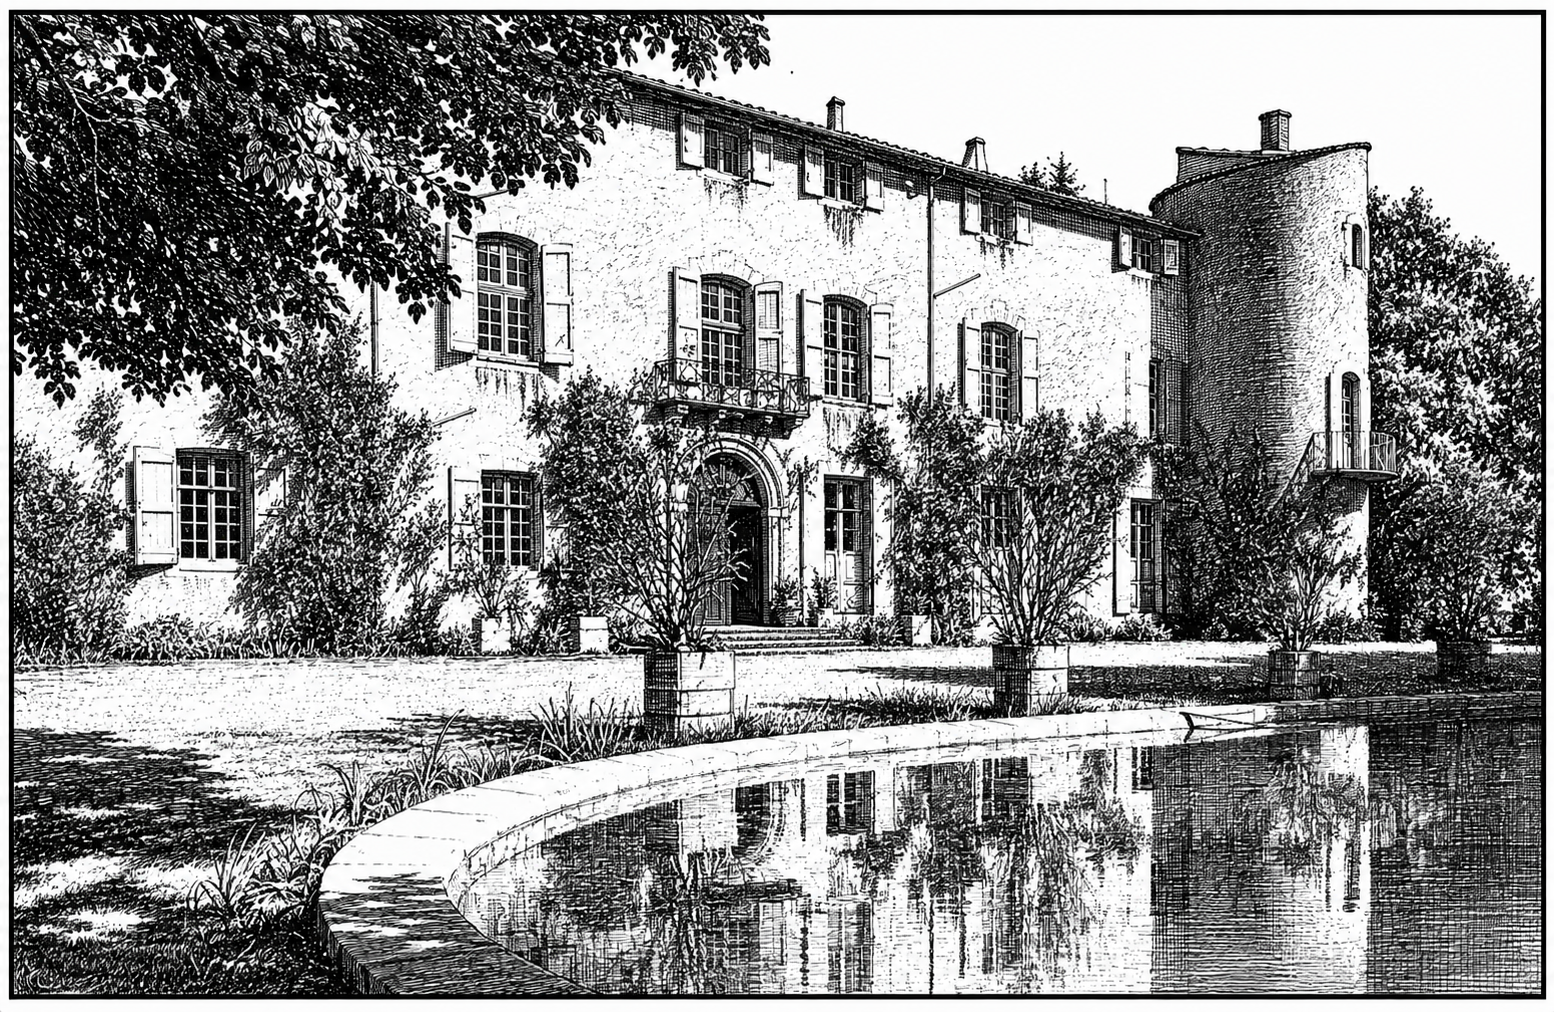
\includegraphics[width=0.78\textwidth]{imgs/071}
\end{center}

% Page 072 — page imprimée 68
% La famille Roussel du Villaret au Château d’Ayres (suite)

\subsubsection{Ginette et Nicole}

\medskip

Ginette Roussel s’était mariée en 1934 ou 1935 avec Jean Teissier du Cros dont la famille,
originaire de Valleraugue, était connue.

\medskip

\textit{(Une des sœurs de Jean, Germaine Dieterlen-Teissier du Cros -ethnologue- devint la collaboratrice de Marcel
Griaule, spécialiste des Dogons, avec qui elle écrivit « Renard pâle », puis l’assistante et compagne de Jean
Rouch ethnologue et cinéaste, auteur de « Moi un Noir »...)}

\medskip

Il avait été en poste en Martinique puis en Chine enfin en Indochine où il emmena sa jeune
femme. Elle n’apprécia sans doute guère la vie « coloniale » ni l’atmosphère de Saïgon. Le
château d’Ayres lui manquait et ils revinrent s’y installer peu de temps avant la guerre. Jean
paraissait de santé délicate, le teint jaune ; il souffrait d’une amibiase chronique dont il ne put
jamais se débarrasser. De pension de familles, le château devint un hôtel réputé sous la
direction ferme de Madame Roussel.

\medskip

Au château était arrivée en 1928, Nicole Roussel qui passait pour être la sœur de Ginette. Elle
était née en 1927, et on disait qu’elle était la fille de Melle Harrison, sœur de Mme. Roussel
qui l’aurait adoptée Elle allait à l’école de filles à Meyrueis et faisait tourner la tête de
plusieurs garçons de l’école contiguë car elle était jolie fille et surtout chantait très bien sans
timidité aucune. Bref, j’en fus amoureux comme quelques autres et plus tard en été 1944 ou
1945 nous nous retrouvâmes dans le groupe de jeunes de la paroisse de Meyrueis pour
quelques balades et réunions diverses.

\medskip

En fait Nicole était, disait la rumeur publique, la fille de Frédéric H\footnote{Frédéric H. voir encadré}, tailleur à Paris, (ou d’un
de ses amis) qu’il avait eue d’une de ses conquêtes parisiennes venue en séjour au château
d’Ayres. Quelques années après, elle épousa un médecin devint Mme. A.. (Mme A mère, était
une Monod) et passa toute sa vie à Châlons sur Marne où elle mourut il y a quelques années.
Elle avait perdu un fils atteint d’un cancer et elle ne s’en était jamais consolée. Son second fils
serait ingénieur en Allemagne

\medskip

.

C’est Ginette qui hérita du château et qui, avec son mari, mais aussi grâce à son maître d’hôtel
– chef du personnel - continua et améliora, la réputation du château qui accueillit quelques
personnalités politiques célèbres telles Adenauer ou de Gaulle ainsi que des artistes connus…

\medskip

Ce maître d’hôtel avait une réputation détestable mais, doué, il avait su se rendre
indispensable. Plusieurs de ceux qui l’ont connu le qualifient encore de « sale bête » (sic).
Protestant, eh oui ! il portait à la ceinture une grosse croix huguenote ancienne. Elle voisinait
avec l’insigne des SAC : les Services d’Action Civique de Charles Pasqua, qui s’illustrèrent
par de nombreuses exactions et sans doute par des crimes. Il ne cachait pas, bien au contraire,
cet engagement politique d’extrême droite !!! Dans le village les jeunes et les enfants
l’avaient surnommé « Casserole ».

\medskip


\noindent
C’est à cette époque, que la chambre de Ginette fut totalement détruite. Sa couverture
chauffante embrasa tout ce qui s’y trouvait ; heureusement elle n’y était pas et les pompiers
parvinrent à circonscrire l’incendie au couloir attenant, mais bijoux, lettres et photos, glaces et
bibelots, tout avait disparu.

\vspace{0.45cm}

Après la mort accidentelle de son maître d’hôtel, Ginette, quelques mois plus tard, tomba
malade et fut emportée par un cancer. Son mari, désormais seul, se résigna à vendre cette
vieille demeure à laquelle il était tellement attaché. Ce fut, pour lui, un crève-cœur. Il tourna
donc définitivement le dos à Meyrueis, Ayres et son château en 1979. Une maison de retraite
l’accueillit aux Sables d’Olonne où il termina sa vie.

\vspace{0.45cm}

C’est désormais la famille de Monjou qui préside aux destinées du Château d’Ayres\ldots

\vspace{1.6cm}

% ------------------------------------------------------------
% Encadré
% ------------------------------------------------------------

\noindent
\fbox{%
\parbox{0.89\textwidth}{%
\small
\textit{%
Frédéric H., de père anglais, tailleur pour hommes, avenue Matignon, ancien combattant
14-18, blessé en 1917, milite dans les Unions Chrétiennes de Jeunes Gens (UCJG).
Sous le couvert de ses activités commerciales et de ses engagements humanitaires où il
soutient des maisons d’enfants, cas sociaux, handicapés\ldots, il peut assez facilement passer la
ligne de démarcation entre la Zone Occupée à la Zone non Occupée et de là se rendre en
Suisse où il s’engage dans un réseau de résistance, le réseau Gilbert, organisé de Genève par
le Colonel Georges Groussard.
Ce Réseau dispose de 700 agents en relation directe avec les services secrets britanniques.
Parmi eux de nombreux « unionistes » Maurice Costil, Charlie Vernier, Le Gal Basteau,
Charles Guillon, Secrétaire International des YMCA (Young Men Christian Association) qui
sont tous plus ou moins convoyeurs de fonds destinés à l’aide aux réfugiés au Chambon sur
Lignon, pour la Cimade etc.%
}
}%
}

\vspace{0.15cm}

\begin{flushright}
Jacques Poujol : « Protestants dans la France en Guerre » p. 228-230
\end{flushright}



\subsubsection{Le moulin d’Ayres}

\vspace{0.55cm}

Nous n’avons que de rares documents nous permettant de retracer les origines du moulin :

\vspace{0.35cm}

A-t-il été construit vers les 11° ou 12° siècle comme beaucoup de moulins en Languedoc ?
Nous l’ignorons. Par contre la photocopie d’un acte retrouvé aux Archives de Mende par
Mme Jeanjean-Sanch, datant de 1574, sous Henri III, vient de m’être remis. Il s’agit d’un
contrat de location du moulin d’Ayres par le seigneur ou le sieur de Fontanille à un certain
Voller ou Valles en cours de déchiffrage en Septembre 2008.

\vspace{0.35cm}

Nous savons également qu’en 1736 il était en pleine activité comme moulin à farine, et il est
répertorié, et lui seul, dans les vallées avec celui de Malbois dans le bourg, sur la carte de
Cassini (1750) mais en 1.900 il n’y avait plus, au Moulin d’Ayres, ni roue, ni meules, !
ni aucun vestige à l’exception :

\vspace{0.3cm}

1/ Du canal d’amenée d’eau encore visible ; il débouche dans la cave de l’aile Sud des
bâtiments actuels ; canal bâti en pierres taillées et ajustées.

\vspace{0.3cm}

2/ D’un acte de « vente » passé devant P.~Berthezène, notaire à Meyrueis à un certain Jean
Rozier, meunier.

\vspace{0.35cm}

A l’époque le moulin ne comportait vraisemblablement qu’un petit bâtiment : le moulin
proprement dit : les meules au niveau de la Jonte et au dessus 2 pièces pour habitation (?).
Il se pourrait que le Rouilladou avec son foulon ait déjà existé.

\vspace{0.35cm}

Le Moulin d’Ayres a donc appartenu à \textbf{Jean Rozier} et à ses descendants jusqu’en 1820.
Le dernier \textbf{Gabriel Rouzier} a vendu le domaine et le moulin toujours en activité, à \textbf{Jean
Louis Laget} comme en fait foi l’acte suivant :

\vspace{0.25cm}

\begin{flushleft}
\hspace{1cm}
\parbox{0.82\textwidth}{
\textit{
« Le 20 novembre 1820 le sieur \textbf{Gabriel Rouzier}, meunier.... a procédé à la vente pure,
simple, à jamais valable, irrévocable avec promesse de faire jouir en paix et d’être en toute garantie
de droit ou d’érection en faveur du sieur \textbf{Jean-Louis Laget}, pour le prix de 4.900 F, un
petit doncs de domaine...
Indépendamment du prix ci-dessus stipulé le sieur Laget demeure chargé de payer à M. de
Montauran, ou à ses successeurs la rente ou pension foncière annuelle perpétuelle de 45,60
Francs ...
Le domaine dispose de 2 jardins indépendants : l’un au devant de la maison d’habitation et se
tenant au chemin qui conduit à la dite maison, l’autre derrière la dite maison et moulin se tenant
d’un côté avec l’aire de l’autre à la dite rivière de Jaonte et du chemin... »}
}
\end{flushleft}

\vspace{0.25cm}

\noindent
\textbf{Jean Louis Laget} était propriétaire foncier à Meyrueis ; a-t-il affermé le moulin sans être
lui même le maître-meunier ? C’est possible. En effet nous savons qu’en 1844 le moulin
était toujours en activité et le meunier, fermier également, à Ayres s’appelait \textbf{Trinchard}.
C’est sans doute vers les années 1850 que les bâtiments furent agrandis pour devenir tels,
ou à peu près, que nous les connaissons aujourd’hui. Ce serait donc \textbf{Jean Louis Laget}
qui aurait financé ces travaux importants.

De 1736 à 1850 environ, le moulin est « bladier » c’est à dire moulin à farine pour le pain,
avec trois paires de meules :

Un moulin « blanc » pour la farine panifiable

Un moulin plus rustique pour les animaux

Un moulin à meule centrale tronconique appelé parfois moulin de l’ase ( moulin de l’âne )
servant à séparer les grains de leur pellicule, comme pour préparer, par exemple, l’orge perlé
( l’orgiat ou gruau ), voire préparer l’huile de noix ou les graines de trèfle, peut-être
également décortiquer les châtaignes séchées de Cabanals ou de Raffègues, voire réduire les
châtaignons en farine couramment panifiée en temps de disette dit E. Le Roy Ladurie... Il
faut se souvenir que le gruau préparé en soupe a été un aliment extrêmement consommé, à
Meyrueis même, dans notre enfance.

\vspace{0.35cm}

C’est en 1843 que le pré du bas, le long de la rivière a été vendu par M. de Montauran à M.
\textbf{Benjamin Pellet} de Meyrueis. Etait-ce le pré du moulin, ou plutôt celui dit « des sœurs » en
aval, appartenant aujourd’hui à Lucien Nazon ? Toujours est-il qu’il avait droit à 14h
d’arrosage par semaine, à prendre 7h. sur chacun des deux jours réservés à la prairie entière.
De même le nouveau propriétaire était tenu d’entretenir la chaussée au dessus de 20 F, lorsque
la remise en état était importante.

\vspace{0.35cm}

Il y eut sans doute de nombreux conflits pour l’usage de l’eau, qu’il s’agisse du Seigneur, du
meunier ou plus tard du filateur. Nous avons connaissance d’un de ces jugements. Il date de
1845. Ce conflit entre Charles de Montauran et Jean Louis Laget, meunier a donné lieu à
procès dont un jugement du tribunal civil de Florac du 10 Mai 1845 nous est parvenu : il a
coûté fort cher aux deux parties : 802 F à M. de Montauran et 401 F. à JL Laget ! Il souligne
la servitude ci-dessus rappelée..

\vspace{0.35cm}

Le moulin « bladier » était aussi un moulin « banier »

Il appartenait au Seigneur d’Ayres et tous les paysans ( le ban et l’arrière-ban ) devaient, sous
peine de poursuites, apporter tous leurs grains au Moulin d’Ayres, au moulin du Seigneur,
qui, évidemment, touchait sa part.

\vspace{1.3cm}

% ------------------------------------------------------------
% Encadré
% ------------------------------------------------------------

\begin{center}
\fbox{%
\parbox{0.72\textwidth}{%
\centering
\small
Le moulin de Gatuzieres n’est plus en activité. Mais il dispose toujours\\
de tout son outillage : deux meules à farine, un cylindre à huile,\\
un tour pour le levage des meules ainsi qu’un tarare\\
pour bluter la farine
}%
}
\end{center}

\subsubsection{La carderie de bourres de soie}


\vspace{0.55cm}

Ce n’est pas sans raisons que \textbf{Jean-Louis Laget} s’était lancé dans ces travaux,
probablement en deux tranches : la partie Sud, jusqu’à la salle d’entrée, puis l’aile
Nord venant rejoindre le foulon (le Rouilladou), tour couverte d’ardoises..

\vspace{0.35cm}

C’est qu’en effet on était en pleine extension de la culture des vers à soie. Il y avait à
Meyrueis de nombreux mûriers et plusieurs élevages contribuaient à l’aisance de
certaines familles. D’où, probablement, l’idée de monter une petite fabrique de
cardage de bourres de soie : les bourres, parties externes du cocon en soie grossière
ainsi que les déchets du dévidage étaient soigneusement récupérés. La fabrique était
alimentée probablement par des bourres de soie venant également des basses
Cévennes, Le Vigan, Anduze, Saint André de Valborgne... et Meyrueis ! (Le registre
des patentes en donne la description suivante) :

\vspace{0.25cm}

\begin{flushleft}
\hspace{0.35cm}
\parbox{0.88\textwidth}{
\textit{
« Le bâtiment principal est mieux bâti et plus important à l’intérieur qu’il ne
paraît l’être du dehors. Il est divisé en quatre compartiments : les deux
principaux renferment les 7 métiers mécaniques, l’un des autres sert de magasin
pour les fris ons et de logement au contremaître et le quatrième qui n’est pour
ainsi dire qu’un hangar sert pour l’étendage des fris ons de filoselle.
Il y a de plus, attenant à la maison une cour assez vaste qui sert aussi pour
l’étendage.
La marchandise, une fois dégrossie est transportée à Meyrueis dans les deux
vastes salles que l’industriel y tient à sa disposition pour être soumise à l’action
des presses. »
}
}
\end{flushleft}

\vspace{0.25cm}

Le contremaître n’est autre qu’un certain Benjamin Avesque à partir de 1850 et
\textit{« sa maison est assez vaste et assez bien bâtie. Les 7 métiers à carder les bourres de soie sont
mus par une chute d’eau de la force de 6 chevaux vapeur actionnant la grande roue
verticale de 5m de diamètre. Cet établissement ne chôme jamais par manque d’eau. »}
(3 métiers servaient à dégrossir les bourres de soie, 4 autres à les « finir », à quoi il faut
ajouter 20 presses à bras.)

\vspace{0.35cm}

Les bourres de soie, une fois cardées et réduites en fins flocons entraient probablement
dans la composition du feutre pour les chapeaux fabriqués à Meyrueis; ou garnissaient
les édredons. On peut penser que le feutre après son passage au foulon ( l’actuel
Rouilladou ) alimentait en partie la Manufacture de Chapeaux de Feutre qui appartenait
aux Couderc frères de mon arrière grand père Louis Couderc dont la fabrique était
située dans les maisons entre la Placette et le Pont Vieux. Leurs descendants sont les
Verdier de Cambonéral à Saint Jean du Gard. Les bourres de soie filées donnaient la
filoselle avec laquelle on fabriquait des gants, des rideaux ,des bas ou des foulards moins
chers qu’en soie naturelle.

\subsubsection{Passage de la soie à la laine}

\vspace{0.55cm}

Jouxtant la « carderie de soie », il y avait donc le foulon exploité par David Saumade

\vspace{0.25cm}

En 1859 le foulon est ainsi décrit : \textit{« Pas de bâtiment, si ce n’est un petit toit sous
lequel sont situées les 2 pots à fouler d’une valeur 400f \hspace{0.5cm} 10\% \hspace{0.5cm} 40 f\\
Valeur du cours d’eau \hspace{2.1cm} 600f \hspace{0.5cm} 5\% \hspace{0.5cm} 30 f\\
Le bâtiment grange \hspace{2.4cm} 200 f \hspace{0.5cm} 5\% \hspace{0.5cm} 10 f. »}

\vspace{0.3cm}

\textit{« ...le foulon est mis en mouvement par une 2° roue également verticale et qui
reçoit une chute particulière... dans les mois les plus secs de l’été les 2 roues
motrices du foulon et des métiers ne peuvent marcher simultanément mais cet
inconvénient est presque nul pour cette usine car elle ne travaille guère que dans
les mois d’automne et d’hiver, époque où l’eau afflue toujours en quantité
suffisante ».}

\vspace{0.35cm}

La carderie de bourres de soie a donc fait place à la filature de laine dans les
années 1859-1861. En 1859 l’exploitant de la « carderie » s’appelait \textbf{Lambert}
mais sur les 7 métiers, 3 avaient été démontés et venaient d’être remplacés par
des métiers à filer la laine et leurs accessoires.

\vspace{0.35cm}

En effet, c’est l’époque où s’est répandue la pébrine, maladie des vers à soie qui
provoqua la ruine de la soierie française et probablement la disparition de
l’élevage des vers à soie dans la région de Meyrueis, d’autant plus que la
fraîcheur des printemps demandait un chauffage onéreux des magnaneries.

\vspace{0.35cm}

\textbf{David Saumade}, exploitant du foulon, achètera le Moulin en 1861.

\vspace{0.35cm}

Il exploitera la filature avec plus ou moins de bonheur, au moins jusqu’à la mort
de sa femme, puisqu’en mars 1888 le moulin fut hypothéqué :

\vspace{0.25cm}

\begin{flushleft}
\hspace{0.35cm}
\parbox{0.88\textwidth}{
\textit{
« ... au profit de M. Jules Germain, filateur domicilié à Florac, en qualité de
légataire universel de Marie Eugénie Germain, décédée, femme du vendeur
pour garantie de reprises dotales de cette dernière se portant à la somme de
2.000 Fr. outre les intérêts conservés par la loi... »
}
}
\end{flushleft}

\vspace{0.25cm}

Incapable de régler cette somme \textbf{Saumade} dut vendre pour « purger cette
hypothèque ». (rembourser à son beau père la dot que ce dernier avait donné à sa
fille lors de son mariage !!!).

Mon arrière grand père, \textbf{Louis Couderc}, tisserand à Meyrueis au Ferradou
connaissant bien Saumade et le Moulin d’Ayres, pour qui il avait travaillé, se
porta acquéreur pour la somme de 9.000 Fr. L’acte de vente fut signé le 26 Mai
1890. (4.000 Fr. furent payés comptant et 5.000 exigibles à la fin Septembre
1893, plus, bien entendu, l’intérêt fixé à 4\% l’an).

\vspace{0.35cm}

C’était une grosse somme et Louis Couderc eut du mal à réunir ces 5.000 Fr.
gagnés par un travail acharné et une vie très austère. (sa fille, Emma Couderc-
Loupiac disait « n’avoir pas toujours mangé à sa faim ») ; au point qu’il
envisagea de revendre le Moulin. Finalement il resta dans la famille, et la
filature fit d’assez bonnes affaires ; la famille connut une certaine aisance
d’autant plus que \textbf{Paul Loupiac}, mari d’Emma, mon grand père, très compétent
avait pris la direction.

\vspace{0.35cm}

Mais la guerre déclarée, en Août 1914 affecta fortement Louis Couderc (son
gendre Paul fut mobilisé dans la territoriale en Ariège et un de ses neveux Albert,
fut tué à la bataille de Soissons en 1915). Louis Couderc avait repris les rênes
mais il mourut en 1917 : ce fut le début du déclin de la filature et de la plupart de
ces petites industries semblables dans les Cévennes.

\vspace{0.35cm}

Elle redémarra cependant en 1918 avec le retour de Paul Loupiac, démobilisé,
mais une première congestion cérébrale en 1926 suivie de plusieurs rechutes
amena l’arrêt définitif de la filature.

\vspace{0.35cm}

Les machines étaient devenues obsolètes : il eût fallu en racheter de nouvelles,
investir et Frank Loupiac le fils qui aurait désiré rester au pays était trop jeune
et sans moyens financiers Peut être se rendit-il compte que ces petites entreprises,
cardages, moulinages, filatures, chapelleries étaient condamnées par « le progrès
industriel ».

\vspace{0.6cm}

\begin{center}
    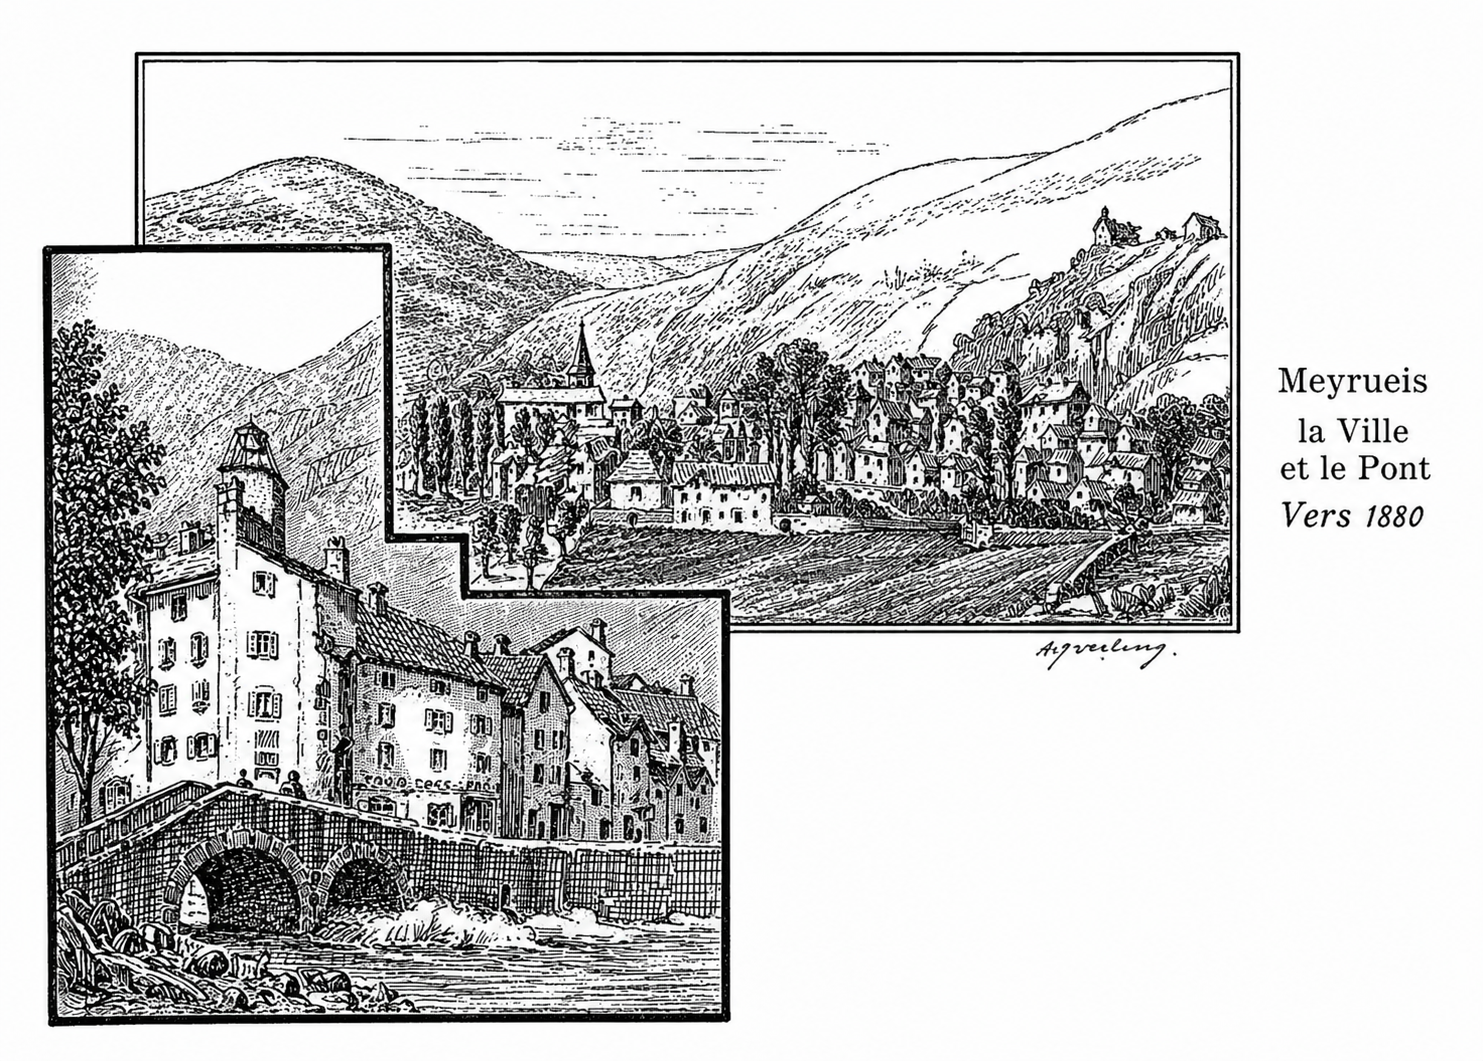
\includegraphics[width=0.9\textwidth]{imgs/078}
\end{center}

% ------------------------------------------------------------
% Page 75
% ------------------------------------------------------------

\begin{center}

\vspace*{0.3cm}

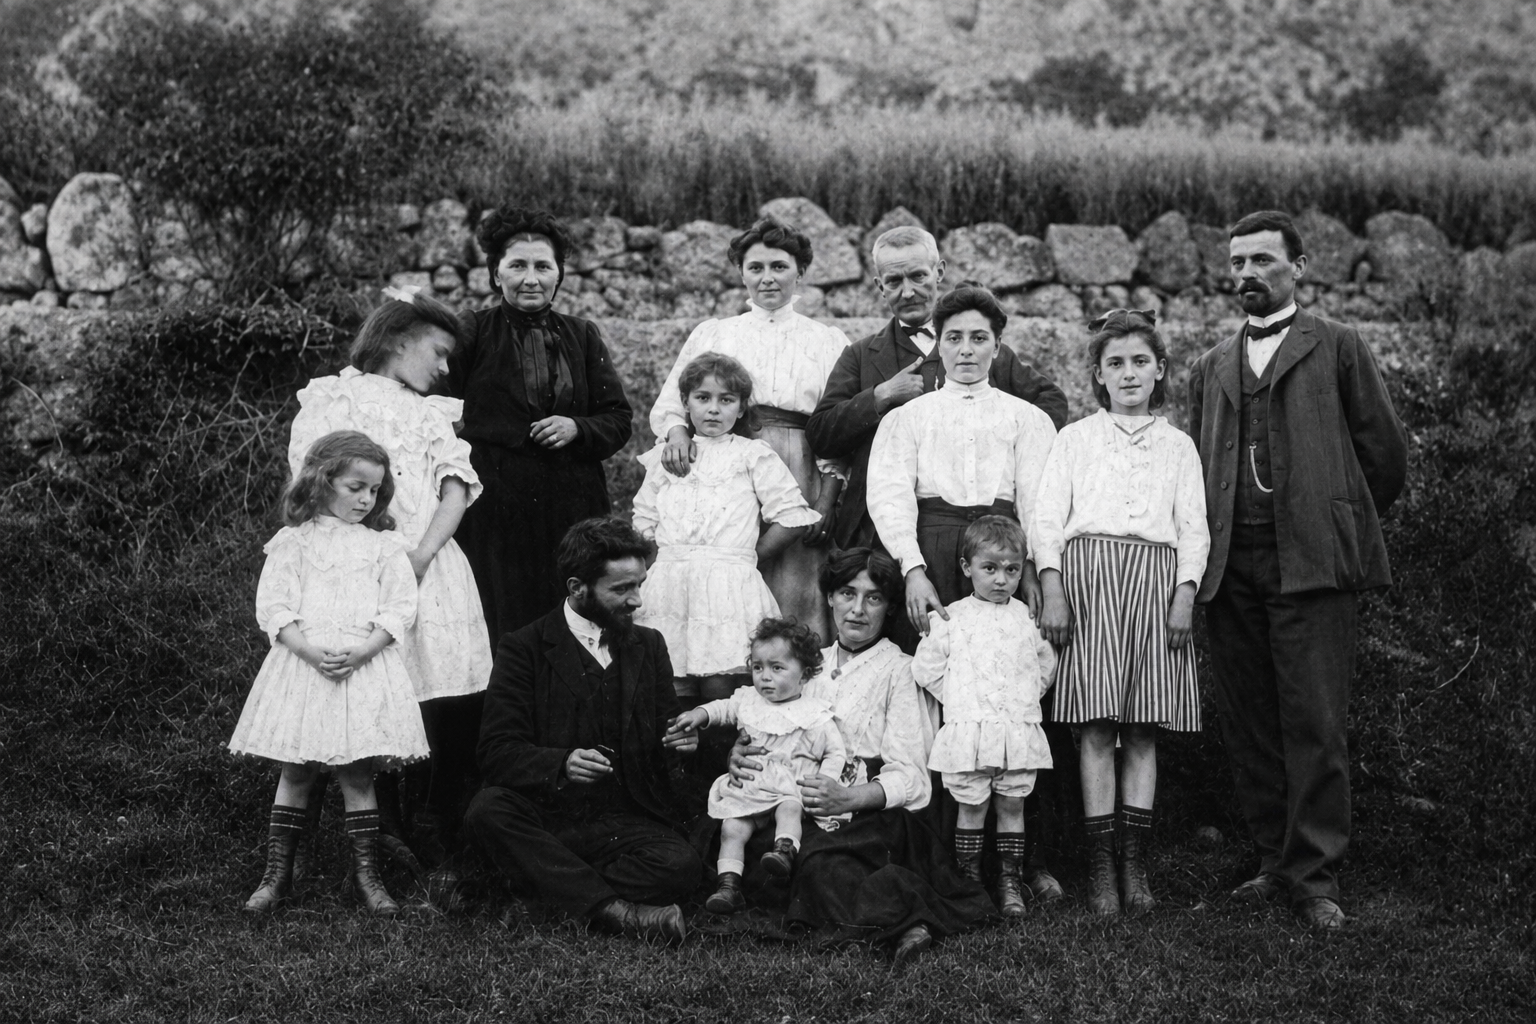
\includegraphics[
    angle=90,
    origin=c,
    width=\textwidth,
    height=0.75\textheight,
    keepaspectratio
]{imgs/079}

\vspace{0.25cm}

{\small
La famille Couderc-Loupiac, Filateurs au Moulin d’Ayres --- 1909
}

\end{center}


\subsubsection{Gatuzieres}


\vspace{0.45cm}

Après le Moulin d’Ayres nous traversons les hameaux de Salvin sac puis de la Bragouse et la
Bragousette pour arriver à Gatuzieres, dominé par les premiers lacets de la route du col de Perjuret.

\vspace{0.3cm}

Petit village où sont regroupées, vers les années 1900, une douzaine de familles avec sa mairie,
son temple construit après la Révolution vers 1840, et son église beaucoup plus ancienne
accompagné d’un très grand presbytère qui fut occupé par quelques sœurs « institutrices » de
l’école catholique Car il y avait, avant les lois de Jules Ferry, deux écoles, une protestante
avec un instituteur et l’autre catholique « tenue » par une ou deux sœurs. Elles laisseront la
place à l’école publique, construite au bas du village et maintenant mairie.

\vspace{0.3cm}

\textbf{Le « château » :} la plus belle propriété qui, de « château » n’en porte que le nom, encore qu’elle
possède un pigeonnier, en ruines aujourd’hui, signe de noblesse. On peut admirer une grange aux
dimensions imposantes avec ses six arcs en ogive dont la construction ne parait pas ancienne. A une
extrémité l’ancien logement du fermier ; celui du propriétaire à l’autre extrémité donne sur un
balcon couvert dont deux piliers proviennent, peut-être, des restes du château. \textbf{Le moulin du Mas
Pradès} --sans doute moulin du château-- fut en activité jusqu’aux années 1960; toutes les meules sont
encore en place. Tous deux étaient situés en aval du village.

\vspace{0.3cm}

A Gatuzieres vivaient quelques petits propriétaires disposant de maigres parcelles de terre et
des journaliers ou bergers engagés par les grosses fermes de la vallée et du Causse Méjean.
Jusqu’aux années 1960 chaque troupeau de brebis était conduit et gardé par un berger drapé
dans sa cape rigide et imperméable et accompagné de son grand parapluie bleu ou rouge,
visible de loin.

\vspace{0.3cm}

Il y avait aussi à Gatuzieres une recette postale avec sa cabine téléphonique. Mme. Dely
Martin tenait le bureau, installée derrière la banque et son grillage. Son mari distribuait le
courrier dans la commune . A sa mort c’est leur fille Alice qui remplaça son père. A 5h00 du
matin elle allait chercher lettres et plis apportés par « le courrier » l’autobus Meyrueis-Florac
qui s’arrêtait bien au dessus du village. Elle montait à Aures puis à Cabrillac, à pied bien sûr
passant par Plambel et Jontanels mais laissant de côté Malbosc desservi par Fraissinet de
Fourques !!! Il lui arrivait de rencontrer le facteur de Rousses qui, lui, avait en charge la
moitié de Cabrillac ( les maisons côté Nord ) !!!

\vspace{0.3cm}

La guerre de 1914 puis celle de 1939-1945 ainsi que la modernisation de l’agriculture
aggravèrent l’exode rural au point que dans les années 1970 il n’y eut plus qu’un seul habitant
permanent au village ; seuls, le moulin du Mas Pradès et le château « lou Castel », dont les
prés habitent désormais un camping, résistèrent.
Le village de Gatuzieres semblait condamné, tout comme Malbosc, Plambel, Jontanels et Cabrillac à
abriter des résidences secondaires préférables, somme toute, à des villages en ruines.

\vspace{0.3cm}

Mais en 1975-1980, un éleveur s’installa à Jontanels ; on vit, à Gatuzieres, se rouvrir
timidement et se réhabiliter quelques maisons. L’installation de la maison de retraite de
Meyrueis puis de petites entreprises ainsi que le Parc des Cévennes, accompagnés du
développement du tourisme avec ses campings et ses gîtes chez l’habitant et le retour de
quelques retraités redonnèrent vie à Gatuzieres où seule une maison en ruine dresse encore ses
pans de murs, sans toit, en plein village !

\vspace{0.35cm}

\begin{center}
    Mais en 2008 Gatuzieres est sauvé !!!
\end{center}

\subsubsection{Cabrillac}

    \vspace{0.15cm}

\begin{center}
    {\large Un hameau sur l’Aigoual}
\end{center}

\vspace{0.45cm}

Cabrillac est le rassemblement de quelques maisons à 1200m d’altitude, écrit Yves Grellier,
sur un sol formant replat, sur le versant nord de l’Aigoual, à quelque sept km. de son sommet
par la route. Il est immédiatement dominé par la draille qui monte droit le long de la
montagne vers le Sud Est. Le village surplombe la haute vallée de la Jonte qui traverse et
arrose de nombreux prés….

\vspace{0.3cm}

Cabrillac est un carrefour sur ce col battu des vents, entre la Jonte et le Tarnon, entre
l’Aigoual et le Causse, entre granite, schiste et calcaire, depuis longtemps lieu de passage des
hommes et des bêtes… Une grande foire annuelle s’y tenait le 20 Mai, foire aux chèvres
comme son nom l’indique, et aux cochons. Les gens du Vigan montent à Cabrillac acheter
leur cochon de l’année qu’ils tueront à Noël…. \footnote{Mme. Poujol dont les petits enfants habitent Montcamp, Meyrueis, Sainte Enimie, etc. préparait la soupe pour les fermiers du Causse Méjean qui venaient faire leur provision de bois dans les forêts de l’Aigoual. Ils arrivaient de Nivoliers ou de la Bégude, de Fretma ou de Gally, d’Aures ou de l’Hom et du Veygaliers…. Les attelages de bœufs traversaient Cabrillac au petit jour. Sans bruit ils ouvraient la porte Poujol (on ne fermait pas les portes en ces temps là) et déposaient dans le tiroir de la grande table un morceau de lard pour assaisonner la soupe des hommes et leur préparer par Mme. Poujol : celle-ci avait coutume de raconter « au morceau de lard je sais quel est le fermier qui va revenir ». Etait-ce à la quantité, à la fraîcheur du morceau, à la façon dont il avait été conservé ? Nous ne savons…}

\vspace{0.3cm}

C’est en 1827 que René de Bernis neveu du cardinal-ministre vend ses terres de Cabrillac à
trois chefs de famille du lieu : Avesque, Poujol et Verdier : familles encore bien représentées
dans le pays, inaugurant ce que l’on a pu appeler l’âge d’or de Cabrillac, mais qui ne dura
qu’une soixantaine d’années.

Pendant trois quarts de siècle de 1870 à 1950 qui aura vu trois guerres ! Cabrillac s’est vidé de
ses travailleurs, de ses enfants, son terroir s’est rétréci, ses troupeaux amenuisés : des vaches
remplacent, en partie, les si nombreuses brebis.

\vspace{0.3cm}

On peut retenir deux dates particulières pour Cabrillac : \textbf{1953} c’est l’arrivée des premiers
estivants urbains qui ont, pour la plupart, une parenté même lointaine avec les Avesque,
Poujol ou Verdier. Ils achètent et retapent de vieilles écuries ou bergeries inoccupées. Une
population nouvelle va remplacer l’ancienne au moins pendant les mois d’été puis de plus en
plus longtemps avec les retraités et l’allongement du temps de la vie.

\textbf{1980} c’est le décès du dernier paysan.

\vspace{0.3cm}

L’hiver Cabrillac est désormais désert.

% ------------------------------------------------------------
% Page 84
% ------------------------------------------------------------

\subsubsection{La tragédie de la Parade}

\vspace{0.35cm}

Le dimanche avant Pentecôte, jour de la fête du Rocher de la Vierge, le maquis Bir Hakeim
avait envahi Meyrueis et désarmé les gendarmes. Le jeune Noguès qui avait 17 ans suivit le
maquis. Je lui avais réglé son compte à l’usine la veille. René Fages (dit Fafa) à qui j’avais
fait la même chose partit également. Le malheureux Noguès une semaine après était pris et
fusillé au col de la Tourette. Fages plus heureux avait réussi à s’échapper (en compagnie de
Pierre Damiani dit Popeye.) Rolland et le pasteur Robert purent les récupérer, blessés,
dans la vallée de la Jonte (tous deux avaient réussi à se traîner jusqu’au Maynial car
Damiani avait été atteint par une rafale de mitraillette au bas du dos) et les planquer au
Moulin d’Ayres près de Meyrueis sur la route de Florac chez Mme. Loupiac.
Notre ami le Dr. Bouisset vint les soigner car Fages avait lui aussi deux balles dans la cuisse.
(En ce qui me concerne je n’ai gardé le souvenir que du Dr. Juliette Caban el venant, dès leur
arrivée (?) leur faire des piqûres antitétaniques tout en ne réussissant pas à extraire une ou
deux balles de leurs blessures. Ils étaient couchés dans la chambre de mes parents au 1er
Etage et chaque jour (?) je venais leur apporter de quoi manger en m’approchant
discrètement faisant semblant de pêcher, car le Moulin restait fermé. Ils restèrent quelques
jours, mais après le passage de la dernière colonne allemande, Rolland et le Pasteur Robert
vinrent les prendre avec la camionnette gazogène pour les cacher chez le Pasteur Chazel à
Vébron. *

\vspace{0.45cm}

Le 6 Juin 1944 une colonne allemande d’une trentaine de véhicules arrivait par la route de
Florac et s’arrêta à l’entrée de Meyrueis (mettant en batterie un petit canon au croisement de
la Fabrique) Sylvain Rey arriva en trombe dans mon bureau disant : « ça y est ! les
américains ont débarqué en Normandie » Sa femme, de l’hôtel, par téléphone, donna l’alerte
concernant l’arrivée des allemands. Aussitôt les irréguliers se retirèrent vers les bois de
Raffègues.
Puis une estafette venue certainement de Mende leur apporta un contre ordre et la colonne
repartit sans avoir exécuté sa mission qui, après ce qui a été dit ensuite devait consister à
arrêter les autorités municipales, à fouiller et à incendier les maisons pour rechercher « les
terroristes »échappés du maquis de la Parade ». Meyrueis l’a échappé belle. (Nous vîmes à
travers les fentes des volets, Damiani, Fafa et moi passer les camions sur la route au dessus
du moulin, s’arrêtant même pour une pose pipi. Quelle frayeur ! ! *

\vspace{0.55cm}

\textbf{Les départs au maquis.}

\vspace{0.35cm}

Peu après ces événements, un matin, en arrivant à l’usine j’appris le départ de Rolland pour le
maquis de l’Aigoual. S’étaient joints à lui son frère « Bonnet », le chef mécanicien ainsi que
4 ou 5 autres réfractaires de l’usine. nos amis le Dr. Bouisset et M. Griscelli, percepteur,
étaient également partis. Restaient pour faire tourner l’usine qui marchait au ralenti M.
Charles, moi même, et quelques ouvriers.

\vspace{0.45cm}

Le maquis vint nous prendre le dernier camion appelé « l’oiseau bleu », le seul véhicule qui
pouvait encore ravitailler Meyrueis. Grâce à une intervention de M. Charles qui put faire
toucher Rolland à l’Aigoual le camion nous fut rendu.

\vspace{0.45cm}

En tout et pour tout nous avons été obligés de livrer à la Kommandantur de Mende, un camion
de charbon de bois. Le chargement avait été tellement bien effectué que dans les virages de la descente de Ste Enimie la plupart des sacs dégringolèrent dans le ravin. Nous ne fûmes jamais
payés.

L’usine redémarra sous un jour nouveau. Il y a lieu de dire qu’en juin les gens d’origine
italienne furent réquisitionnés par le STO. C’est ainsi que notre excellent chauffeur Persico,
bien que naturalisé français dut partir : même chose pour ce pauvre Pugnale Gino dont le fils
était infirme.

\vspace{0.45cm}

Fin juillet ou début Août après la libération d’Alès et de Nîmes ceux qui avaient pris le
maquis revinrent à l’usine. Ils avaient bien combattu dans la région du Vigan, Ganges et Saint
Hippolyte, retardant les colonnes allemandes sur la nationale 99.

\vspace{0.55cm}

\textbf{Après la libération}

\vspace{0.35cm}

Après la fin de cette période d’incertitude où tout le monde était sur le qui-vive j’interrogeais
tous ceux qui s’étaient fait inscrire sous un nom d’emprunt. Je fis un état que j’envoyais à la
Sécurité Sociale à Mende pour signaler que les cotisations versées sous le nom de M. X
concernaient en réalité M. Y ... né à ... etc... Ainsi les cotisations versées ne furent pas
perdues. Sur un effectif de 35 personnes travaillant en usine pendant cette période 1943 –
1944 la moitié était en situation irrégulière :

\vspace{0.25cm}

Evadés d’Allemagne Prisonnier de Guerre \hfill 1

-------------------S T O \hfill 1

Requis évadés ou ne s’étant pas présentés \hfill 12

Planqués avant d’être requis \hfill 6

\vspace{0.4cm}

Ces chiffres je les donne avec réserve et je les base sur des souvenirs en faisant appel à ma
mémoire. Je pense qu’ils doivent être à peu près exacts.
Travaillaient en forêt le contremaître forestier Neufeld et des équipes de bûcherons. L’effectif
forestier était d’une quinzaine. Parmi eux se trouvaient également des garçons évadés du
STO.

\vspace{0.55cm}

\textbf{L’usine de Carburants Forestiers et Meyrueis}

\vspace{0.35cm}

L’usine a rendu de très grands services à la population de Meyrueis. Rolland lorsqu’il
descendait à Millau ou à Nîmes emmenait toujours quelqu’un dans la voiture de liaison.
Lorsque les camions revenaient de livrer du charbon de bois ils aidaient au ravitaillement. Il
s’était créé également des liens de solidarité parmi tout le personnel. Il n’y eut aucune
dénonciation bien qu’il y eut dans l’usine, 3 ouvriers qui, par bêtise, s’étaient fait inscrire à la
Milice, soi-disant pour ne pas partir en Allemagne bien qu’à l’usine existât cette garantie !!! ;
mais n’en bénéficièrent pas les étrangers !

\vspace{0.55cm}

\textbf{La page est tournée.}

\vspace{0.35cm}

Notre usine des Carburants Forestiers a tenu encore pendant 5 ans après la libération. Elle
s’était orientée vers d’autres fabrications mais par suite de l’éloignement et de complications
administratives elle fut obligée de déposer son bilan.

% ------------------------------------------------------------
% Page 86
% ------------------------------------------------------------

Lorsque l’on passe sur la route de Meyrueis à Campis on peut voir les ruines de ce qui fut
l’usine des Carburants Forestiers. Les vestiges de 2 fours subsistent encore. Un corps de
bâtiment sert d’écurie pour les chevaux destinés aux promenades. Les jeunes ignorent tout de
cette époque mais nous, les anciens qui l’avons vécue ne pouvons pas oublier.

\vspace{0.8cm}

\begin{flushright}
Le 10 Juillet 1984\\
Robert Cabanel
\end{flushright}

\vfill

\textit{Ce texte a été saisi ( comme on dit maintenant) par Paul Loupiac le 17 Septembre 2002 ;}

\vspace{0.3cm}

\textit{Il m’avait été remis par Georges Rolland en été 2000. Je me suis permis d’ajouter, pour une lecture
plus aisée}

\vspace{0.3cm}

\textit{Les têtes de paragraphes en Gras}

\vspace{0.3cm}

\textit{* Quelques notes --en italique -- qui complètent ou rectifient le témoignage de Robert Cabanel puisque
j’étais à Meyrueis au printemps 1944 et au moulin d’Ayres le 6 Juin ?. Elles montrent combien on
oublie, combien notre mémoire est sélective, et combien certains épisodes nous ont frappé et pas
d’autres. D’où l’importance de témoignages multiples pour les mêmes aventures ou les mêmes
événements.}



\subsection{La  vallée de la Brèze}

La Brèze se jette dans la Jonte, un peu en amont de Meyrueis, après la piscine et près du
vieux pont désaffecté maintenant. Jusqu’aux années1950 il était dominé par le fameux « arbre
du poivre » que tout le monde connaissait, témoin de bien des jeux d’enfants, de serments
échangés à son ombre comme des heures tragiques que connut notre ville :

\vspace{0.65cm}

\begin{center}
    {\large\bfseries L’ARBRE DU POIVRE}
\end{center}

\vspace{0.45cm}

\begin{center}
\begin{minipage}{0.55\textwidth}
L’arbre du poivre est mort, témoin majestueux\\
Des siècles écoulés. Les flots tumultueux\\
De la Brèze irritée, à son pied tutélaire\\
Ne viendront plus briser l’élan de leur colère.

\vspace{0.35cm}

L’arbre du poivre est mort, il avait vu passer\\
Les héros, qu’un vain roi voulait faire chasser\\
Parce qu’ils priaient Dieu, sans obéir à Rome\\
Sous ses branches, parfois, ils chantaient leurs psaumes,

\vspace{0.35cm}

Ou lorsqu’ils descendaient du roc des protestants\\
Contre son tronc noueux, s’adossaient un moment\\
Disant à demi voix leurs projets téméraires\\
De prêcher au Désert, au risque des galères.

\vspace{0.35cm}

L’arbre du poivre est mort. Les générations,\\
Passent comme un éclair, leurs révolutions\\
Le laissent calme et froid. A son cœur insensible,\\
Les siècles passaient des jours purs et paisibles

\vspace{0.35cm}

Naguère, encore debout dans sa sérénité\\
Il était vigoureux comme en son plein été,\\
Il paraissait doué d’éternelle jeunesse\\
Il semblait à l’abri des coups de la vieillesse

\vspace{0.35cm}

Des atteintes de l’âge il était triomphant\\
Tel que l’avaient toujours connu nos yeux d’enfants\\
Sans cesse rajeuni d’une sève vivante\\
Il élancait au ciel ses branches verdoyantes.
\end{minipage}
\end{center}

\vfill

\begin{flushright}
\textbf{…/…}
\end{flushright}

\newpage

\begin{center}
\begin{minipage}{0.55\textwidth}

On venait l’admirer, ce noble et fier géant,\\
Les touristes lassés, s’asseyaient sur son banc\\
Placé près du vieux pont, pour contempler à l’aise\\
Le site séduisant du vallon de la Brèze.

\vspace{0.35cm}

Nous l’aimions, il était le vaste souvenir\\
De notre enfance heureuse, et n’aurait dû mourir\\
Que longtemps après nous, pour parler de nos vies\\
Aux fils de nos enfants, jouant dans sa prairie

\vspace{0.35cm}

Mais un passant tardif, du sort, vil ouvrier\\
A débroussé sa pipe au pied du poivrier\\
L’étincelle a gagné le cœur du sycomore\\
Et le feu l’a rongé, subtil, jusqu’à l’aurore.

\vspace{0.35cm}

Il était beau ! Qu’importe, il lui fallait périr\\
Il était grand, hélas quand la voix implacable\\
Du trépas nous condamne, il nous faut obéir\\
Tous, tant grands que petits, à l’ordre inexorable.

\vspace{0.35cm}

Mais au printemps prochain quelques rejets\\
Renaîtront vigoureux de ses cendres immenses,\\
Et le destin vengeur de l’acte du pervers\\
Saura lui ménager une longue existence.

\vspace{0.35cm}

La même sève ardente, en ses mille canaux\\
Coulera sans arrêt pendant plus de cent lustres\\
Et que le vieux poivrier vivra dans les rameaux\\
D’un puissant sycomore, à son tour très illustre

\vspace{0.35cm}

Ainsi, bientôt, pour nous la vie aura pris fin\\
Mais la sève, abandonnant les restes\\
De son corps périssable à son heureux destin\\
Fera revivre un corps glorieux et céleste.

\vspace{0.55cm}

\textit{Meyrueis le 30 Octobre 1928}\\
\textit{Signature presque illisible : un nommé REY ? ? ?}

\end{minipage}
\end{center}

\vfill

\begin{flushright}
\textit{Poème trouvé dans les archives}\\
\textit{de Marceline Causse}\\
\textit{à Pradines}\\[0.15cm]
Octobre 2002
\end{flushright}

% ------------------------------------------------------------
% Page 79
% ------------------------------------------------------------

\thispagestyle{empty}

\begin{figure}[p]
    \centering

    % Photo du haut
    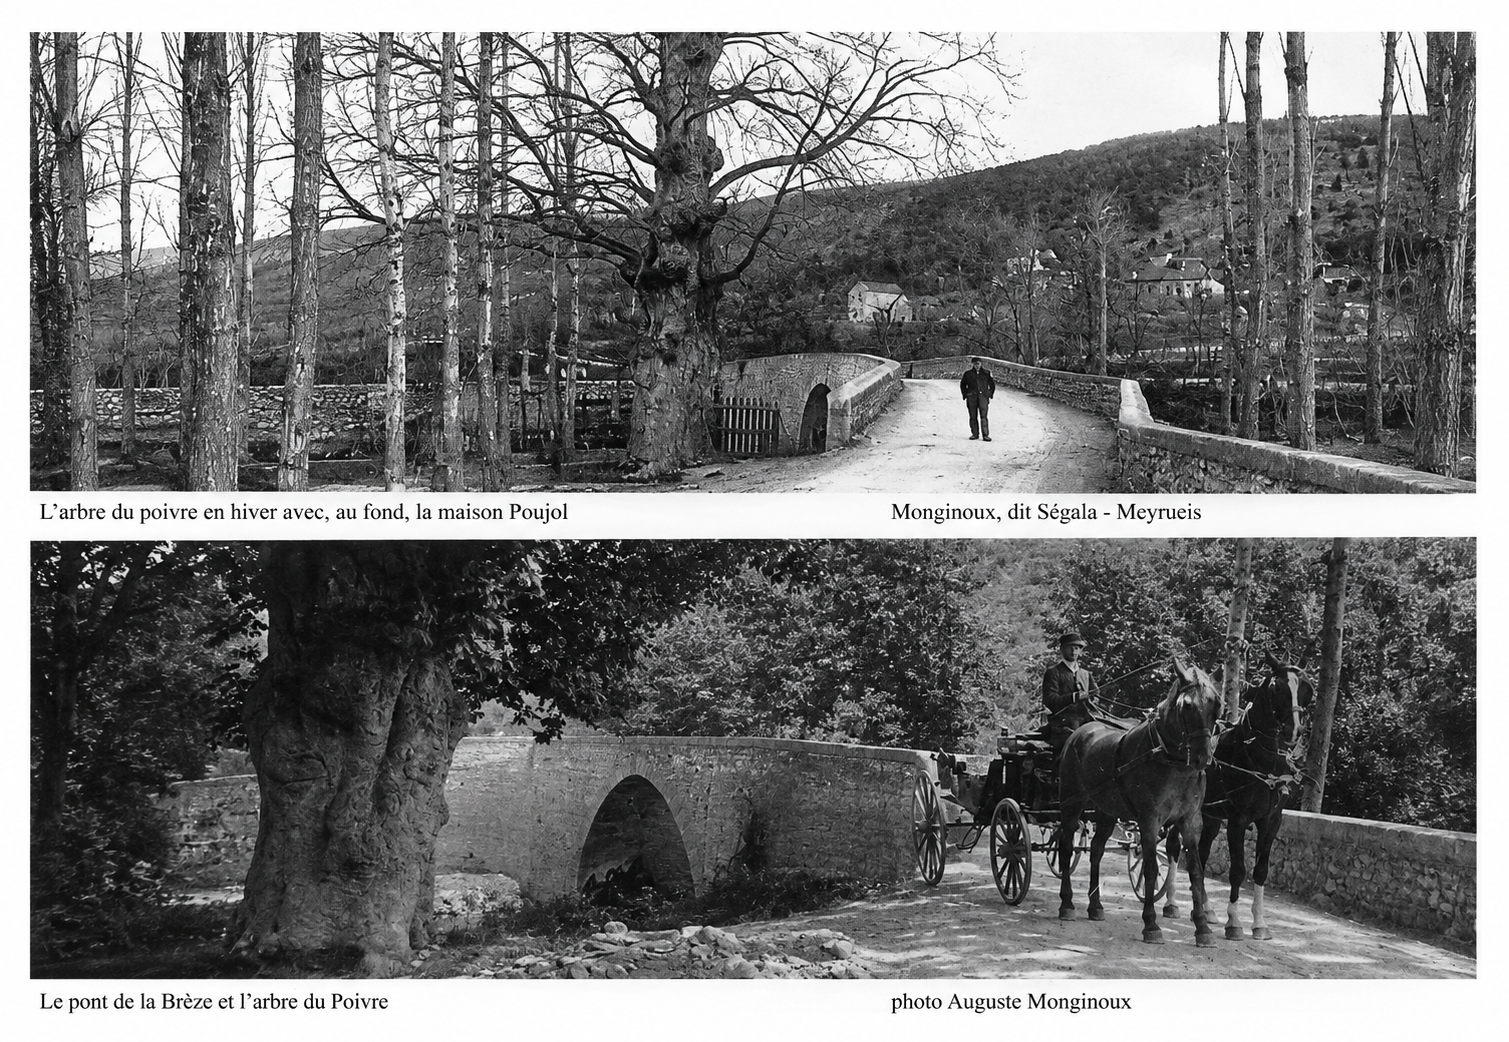
\includegraphics[
        width=\textwidth,
        height=0.47\textheight,
        keepaspectratio
    ]{imgs/084-1}

    \vspace{0.15cm}

    \begin{minipage}{\textwidth}
        \small
        \raggedright
        L’arbre du poivre en hiver avec, au fond, la maison Poujol
        \hfill
        Monginoux, diapositive, Meyrueis
    \end{minipage}

    \vspace{0.35cm}

    % Photo du bas
    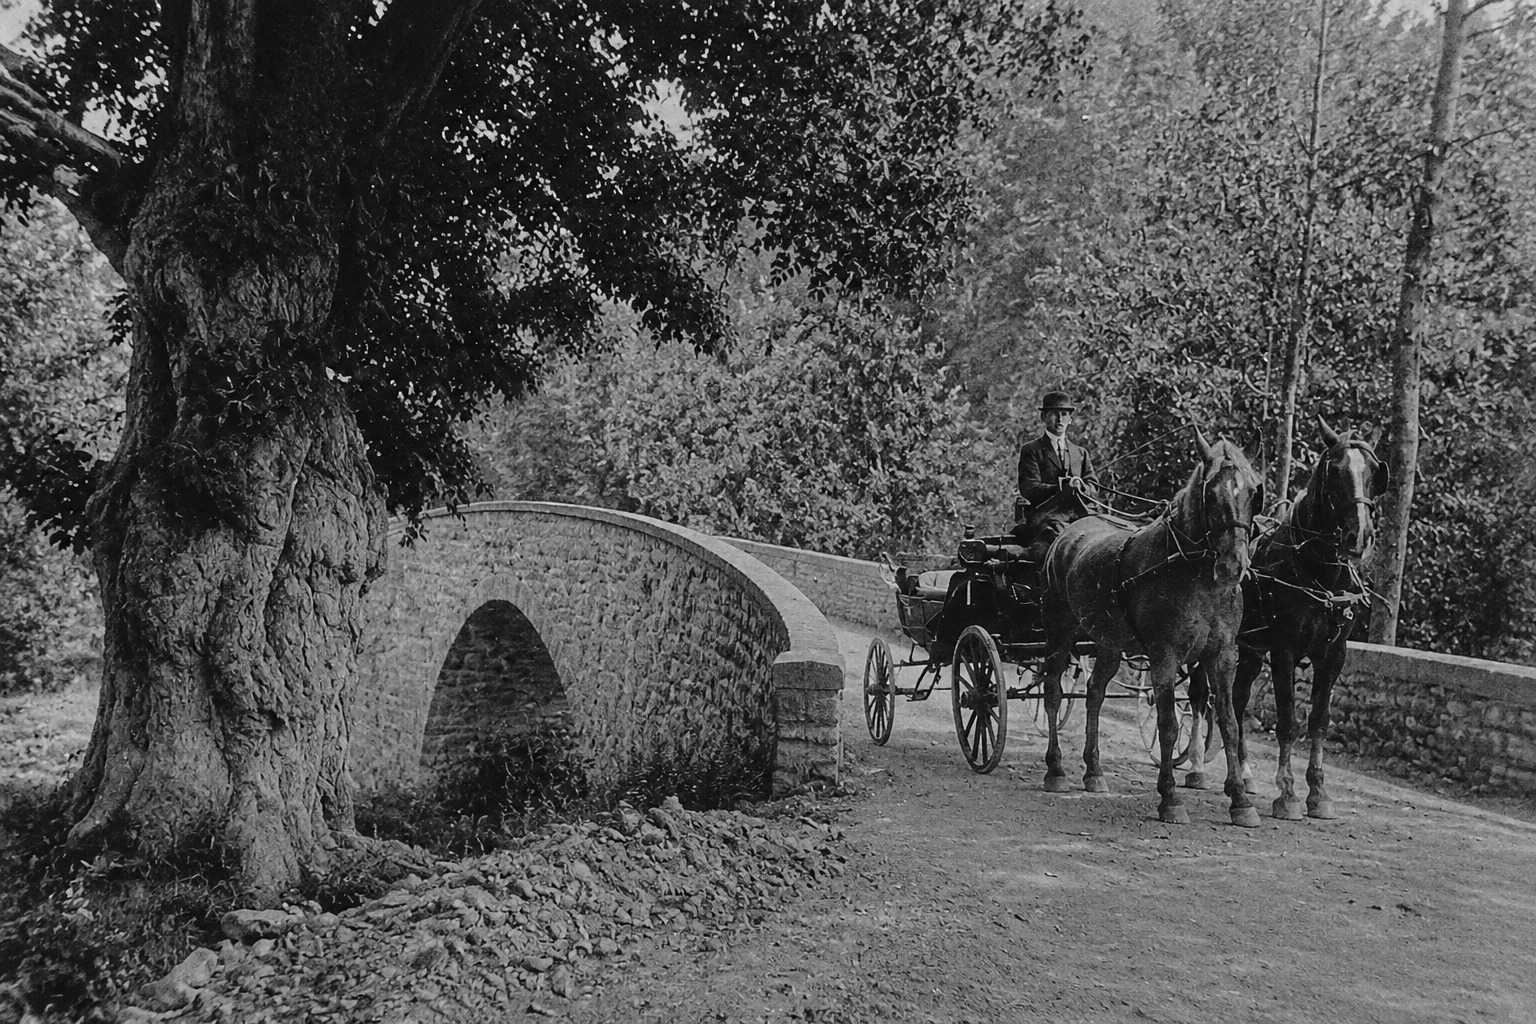
\includegraphics[
        width=\textwidth,
        height=0.43\textheight,
        keepaspectratio
    ]{imgs/084-2}

    \vspace{0.10cm}

    \begin{minipage}{\textwidth}
        \small
        \raggedright
        Le pont de la Brèze et l’arbre du Poivre
        \hfill
        photo Auguste Monginoux
    \end{minipage}

\end{figure}

\clearpage

% ------------------------------------------------------------
% Page 79
% ------------------------------------------------------------

\subsubsection{La Société Cévenole de Carburants Forestiers}


\vspace{1.2cm}

L’histoire de la Société Cévenole des Carburants Forestiers, qui fut créée, près de
Meyrueis, pendant l’hiver 1942, est exemplaire. Il s’agissait, grâce à un brevet suisse,
de produire un charbon de bois adapté aux gazogènes. La construction des fours fut
entreprise au lieu-dit Alauze, à deux km de Meyrueis, dans la vallée de la Brèze. Le
directeur Georges Roland et le comptable Robert Cabané, ne tardèrent pas à recruter
de nombreux jeunes désireux de travailler et d’échapper au STO (Service du Travail
Obligatoire), comme le leur permettait le classement officiel de la Société Cévenole en
tant qu’« usine prioritaire ».

\vspace{0.45cm}

L’un des premiers à s’embaucher fut un réfractaire rescapé d’Aire de Côte. (maquis
installé à la Maison Forestière d’Aire de Côte, non loin de l’Aigoual, décimé par une
attaque de chasseurs parachutistes allemands le 1\textsuperscript{er} Juillet 1943).
Puis ce furent sept ou huit polonais placés en résidence surveillée à l’Hôtel de France.
Des membres de la famille du directeur, un prisonnier évadé, des requis nîmois du STO,
deux Alsaciens, vinrent les rejoindre, tous bénéficiant des cartes de ravitaillement
obtenues par des contacts personnels auprès des services gardois compétents.

\vspace{0.45cm}

Dans certains cas, l’inscription sur les registres d’embauche était fictive et servait de
couverture aux bénéficiaires. Dans d’autres cas, au contraire, des réfractaires trop
exposés faisaient le travail sans être inscrits sur les registres. « Quelle gymnastique
de chiffres ! » nous dit le comptable chargé de faire viser le livre de paye à Mende.
C’est ainsi que, sur les trente cinq employés réguliers de la Société Cévenole,
presque une vingtaine peuvent être considérés comme des « réfugiés » plus ou moins
clandestins.

\vspace{0.45cm}

Mais cette « planque » connut aussi plusieurs drames. Dans la nuit du 29 au 30 mars
1944, des camions allemands vinrent enlever les Polonais de l’Hôtel de France et
l’on n’entendit plus parler d’eux.

\vspace{0.45cm}

Parmi les employés, le jeune Noguès, qui avait cessé le travail pour suivre le maquis
Bir Hakeim, fut capturé à la Parade et fusillé. Un autre employé de la Société
cévenole, le jeune Fages, qui s’était aussi engagé à Bir Hakeim, fut grièvement
blessé au combat, recueilli dans la vallée de la Jonte, où il avait pu se traîner,
transporté dans la voiture de liaison de l’usine et soigné, d’abord au Moulin d’Ayres
chez les Loupiac, puis à Vébron, chez le pasteur Chazel.

\vfill

\begin{flushright}
Cévennes terre de refuge 1940-1944\\
Presses du Languedoc P. 290-291
\end{flushright}

\clearpage

% ------------------------------------------------------------
% Page 80
% ------------------------------------------------------------

\begin{center}
    {\Large\bfseries
    LA SOCIETE CEVENOLE DES CARBURANTS\\
    FORESTIERS
    }

    \vspace{0.7cm}

    {\Large\bfseries
    A MEYRUEIS
    }

    \vspace{0.9cm}

    Témoignage sur son action pendant l’occupation\\
    par Robert Cabanel, ex – comptable à l’Usine
\end{center}

\vspace{1.1cm}

La pénurie d’essence, à cette époque, avait orienté les recherches en carburants de
remplacement. Le charbon de bois faisait tourner les moteurs à gazogène. Un brevet suisse,
exploité en usine à Chapareillan près de Grenoble ayant donné de bons résultats, incita les
dirigeants à monter d’autres usines. C’est ainsi qu’après avoir visité le massif forestier de
l’Aigoual, les dirigeants de l’usine de Chapareillan se mirent en rapport avec un groupe
financier de Nîmes ayant à sa tête la banque Arnaud et Gaidan et décidèrent de monter une
usine à Meyrueis. La Société Cévenole des Carburants Forestiers fut constituée avec Meyrueis
comme siège social.

\vspace{0.45cm}

\textbf{Les débuts de l’Usine d’Alauze}

\vspace{0.35cm}

La construction démarra en hiver 1942 sur un terrain situé au lieu dit Alauze, à deux km de
Meyrueis dans la vallée de la Brèze. La forêt était à une quinzaine de km. Il s’agissait donc de
fabriquer du charbon de bois en usine dans des fours : les sous – produits, goudrons et jus
pyrolygneux étaient récupérés et, après une certaine préparation, on arrivait à fabriquer des
agglomérés de charbon de bois sous forme d’ovoïdes dont le rendement dans les gazos était
supérieur au charbon de bois ordinaire.

\vspace{0.45cm}

Je dois dire que j’étais, depuis le 6 Septembre 1941, Greffier de la Justice de Paix de
Meyrueis.. Situation de rencontre nécessitée par les circonstances du moment. En effet, après
avoir été mobilisé au 104\textsuperscript{o} bataillon de chasseurs alpins j’avais eu la chance, en faisant partie
de l’armée des Alpes, de pouvoir rentrer dans mon foyer à Cannes où j’exerçais depuis 10 ans
la profession d’employé de banque. La situation économique allait en se dégradant. Des bruits
les plus pessimistes circulaient. On parlait d’envoyer bientôt des Français travailler en
Allemagne. Les employés de banque et les employés d’assurance semblaient les plus visés.
Ma femme attendait notre 2\textsuperscript{o} enfant. Je ne voulais à aucun prix partir en Allemagne et
j’acceptais donc la proposition de mon père, retiré à Meyrueis, consistant à acheter le Greffe
de la Justice de Paix qui allait être vacant et à venir travailler quelques parcelles de notre
petite propriété de Pradines. Après les démarches administratives assez longues, j’obtins
l’autorisation de déménager au titre du « Retour à la Terre » préconisé par le régime de
Vichy.

\vspace{0.45cm}

Quitter Cannes pour Meyrueis constituait pour nous un double sacrifice :

En effet j’abandonnais un traitement de 1.800 F par mois pour une indemnité de fonction de
Greffier de 530 F par mois.

D’autre part la côte d’Azur avec la douceur de son climat et la petite villa confortable que
nous habitions n’avaient rien de comparable avec notre maison de campagne de Pradines.

\clearpage

% ------------------------------------------------------------
% Page 81
% ------------------------------------------------------------

La perspective d’un ravitaillement meilleur, avec les possibilités de culture et une plus grande
sécurité nous firent opter pour cette solution. Nous venions d’avoir notre 2\textsuperscript{o}
enfant lorsqu’en Août 1941 nous quittâmes la Côte d’Azur.

\vspace{0.45cm}

J’entrais en fonction peu après. Mon travail de Greffier m’occupait environ 10 (?) heures par
mois. Je consacrais le reste de mon temps à la propriété. Cela dura ainsi jusqu’au printemps
1943. C’est alors que j’appris que l’usine de Carburants Forestiers embauchait du personnel
et qu’elle allait bientôt démarrer.

\vspace{0.45cm}

Connaissant la comptabilité, je me présentais comme comptable. Je fus accepté par le Conseil
d’Administration qui acceptait que je prélève 2h par mois pour la tenue des audiences de la
justice de paix.

\vspace{0.45cm}

Je pris donc mes fonctions le 1\textsuperscript{er} Juillet 1943. L’usine n’était pas tout à fait achevée. On
constituait le stock de bois. Je fus, au cours de ce mois de juillet envoyé en stage à
Chapareillan en Isère, pendant une semaine.

\vspace{0.45cm}

Début Août 1943 l’usine était prête pour les essais. Le Directeur était un jeune ingénieur des
Arts et Métiers M. Georges Rolland, son adjoint un dessinateur projeteur M. Charles. Nous
avions à l’époque de 28 à 33 ans. J’étais le plus âgé. Nous sommes depuis devenus
d’excellents amis.

\vspace{0.45cm}

\underline{Le PDG adjoint M. Fouilloux m’avait dit que nous étions classés usine prioritaire, que nous aurions à livrer une partie de notre production aux Allemands et que cela dispensait tout le personnel du STO. Avantage fort appréciable.}

\vspace{0.55cm}

\underline{\textbf{L’attaque du maquis d’Aire de Côte en 1943}}

\vspace{0.35cm}

\underline{L’affaire} d’Aire de Côte s’était passée le 1\textsuperscript{er}. juillet, \textit{( il semble qu’il y ait erreur car ce
maquis fut attaqué en mai 43 avec 7 morts et 39 prisonniers déportés )} jour de mon
embauche. Plusieurs réfractaires eurent la chance de pouvoir s’échapper. L’un d’eux s’était
réfugié à Ayres. Il vint se faire embaucher après avoir pris contact avec le pasteur Robert. Je
l’inscrivis sous le nom de Guigues.

\vspace{0.45cm}

Pour toute embauche, il fallait remplir une fiche avec tous les renseignements d’identité
concernant le candidat et l’emploi qu’il devait occuper. Cette fiche était envoyée au STO à
Mende qui donnait son autorisation. Il nous était interdit d’embaucher sans autorisation du
STO.

\vspace{0.45cm}

Je me souviens du repas d’inauguration offert par la Direction. Il eut lieu un des premiers
dimanches d’Août 1943. Notre ami « Marius » qui assurait les liaisons et le ravitaillement des
bûcherons s’était arrangé pour nous faire faire un excellent repas dans l’entrée de l’usine. Il y
avait un garçon embauché comme chef de four sous le nom d’Alleyard ou Tallevard. J’avais
enregistré contre lui un PV de Gendarmerie pour une contravention bénigne ; il ne s’était pas
présenté à l’audience. Les gendarmes le recherchaient comme réfractaire au STO. Il en fût
averti et mon camarade Sylvain Rey, hôtelier à Meyrueis vint me dire : « Ce garçon est traqué dépêche toi de lui régler son compte ». ce que je fis bien que l’on fût un dimanche.
Effectivement 2 jours après nous eûmes la visite des gendarmes qui recherchaient ce garçon.

\vspace{0.45cm}

L’usine commençait à tourner, mais dans des conditions épouvantables. Les pannes se
succédaient. Il fallait toute l’astuce et l’imagination de Rolland et de son adjoint pour arriver à
résoudre les problèmes les plus urgents. Il fallait descendre à Nîmes avec un mouton pour
avoir des pneus synthétiques, un gigot pour avoir des pointes ou des pièces de rechange. Les
aciers ne valaient rien ; tout cassait. La route allant en forêt était épouvantable. Les chauffeurs
dont notre ami Persico descendaient leurs 5 tonnes de bois à raison de 2 voyages par jour dans
des conditions inimaginables.

\vspace{0.45cm}

Au début de l’automne 1943 l’Hôtel de France à Meyrueis fut réquisitionné par la Préfecture.
On vit arriver un groupe de polonais placés en résidence surveillée. Le STO nous autorisa à
embaucher ceux qui voulaient travailler. Nous ignorions les origines de ces gens, 7 ou 8
vinrent travailler. Je me souviens de l’un d’eux d’assez forte corpulence qui s’appelait Pakula.
Il parlait assez bien le français.

\vspace{0.45cm}

Vers le milieu de l’hiver 1944, M. Rolland qui revenait d’un voyage à Nîmes me dit qu’il
venait d’embaucher un jeune technicien, élève à l’école des Arts et Métiers qui s’appelait
« Bonnet » ainsi qu’un autre qui répondait au nom de « Séguret ». Une heure après alors que
j’étais seul dans mon bureau Rolland vint me dire à mi-voix et en me regardant bien dans les
yeux : Caban el ! Bonnet c’est mon frère prisonnier évadé d’Allemagne et Séguret c’est mon
cousin germain. Ce dernier requis par le STO s’était accidentellement cassé une jambe en
Allemagne. Après une hospitalisation de 2 mois il avait bénéficié d’un congé de
convalescence de 10 jours. Sur le point de repartir Rolland l’avait engagé à venir se camoufler
à l’usine de Meyrueis. Bien sûr, j’assurai Rolland de la plus grande discrétion. Peu après
j’assistai à la rencontre des deux cousins dans mon bureau, l’un demandant à l’autre
« Comment t’appelles-tu maintenant ? ».

\vspace{0.45cm}

Des parents du PDG de la Cévenole qui avaient une vingtaine d’années vinrent se faire
embaucher pour éviter le STO. Ils arrivaient de Nîmes qui était occupée par les Allemands.
D’autres, du même âge, venaient d’Avignon. Il y avait le fils d’un armurier de cette ville.

\vspace{0.55cm}

\textbf{Réfractaires et Etrangers à l’usine}

\vspace{0.35cm}

D’autre part il y avait un jeune mécanicien appelé Ausset. Son père était chef de service au
Ravitaillement à Nîmes. Par lui Rolland put se procurer des cartes d’alimentation pour les
irréguliers. Il y avait aussi un contre maître nommé Carrier Victor venu de Chapareillan pour
éviter le STO.

\vspace{0.45cm}

Plus tard le PDG de Nîmes nous envoya un autre réfractaire, Joseph Mondino, d’origine
niçoise. Il travaillait comme metteur au point des moteurs d’avion à Marignane. Les
allemands ayant envahi son usine, il put miraculeusement s’échapper et fut dirigé sur
Meyrueis. Nous avons à ce jour conservé d’excellentes relations d’amitié. Joseph Mondino
déployait des trésors d’imagination pour faire tourner les moteurs fatigués. Le contremaître
forestier s’appelait Neufeld. Il était marié, originaire d’Obernai en Alsace. Il s’était échappé
et avait pu, après avoir effectué un temps aux Chantiers de Jeunesse, se faire embaucher.

\vspace{0.45cm}

Rolland qui a tout fait pour rendre service ,en camouflant tous ceux qui étaient traqués, en
était arrivé à la situation suivante :

% ------------------------------------------------------------
% Page 83
% ------------------------------------------------------------

Un petit nombre travaillait sans autorisation du STO en attendant une identité d’emprunt.
(Ceux pour lesquels on n’avait pas pu faire autrement).

\vspace{0.45cm}

D’autres s’étaient fait inscrire sous une identité d’emprunt. Il y en eut deux, dont un de
Vébron qui ne travaillèrent jamais mais dont on avait demandé l’autorisation d’embauche.
Tout cela posait un très sérieux problème administratif ; j’avais proposé, pour le résoudre, de
faire un livre de paye de circonstance pour le STO où j’inscrivais les salaires fictifs ou pas de
tous les inscrits.

\vspace{0.45cm}

Il fallu deux fois aller à Mende pour faire viser le livre que j’avais paraphé moi-même avec le
sceau de la Justice de Paix de Meyrueis que je détenais comme Greffier. C’est notre ami
Sylvain Rey, hôtelier à Meyrueis qui s’était fait embaucher comme chef de vente qui allait à
Mende faire viser le livre de paye. Il le faisait avec beaucoup d’assurance. Quelle
gymnastique de chiffres pour arriver à cadrer avec la Caisse.

\vspace{0.45cm}

Un matin de cet hiver 1944 alors que je quittais notre maison de Pradines située à 1,5 km du
village je vis deux sentinelles allemandes sur le pont de Roquedols. Ils me laissèrent passer. A
l’entrée de Meyrueis même chose. En passant devant l’Hôtel de France je vis un camion Les
allemands embarquaient les polonais. Je continuais mon chemin vers l’usine. Arrivé à la
hauteur du rocher d’Alaouze qui surplombe la route je vis tomber un petit caillou devant mon
vélo. Levant la tête j’aperçus le groupe des irréguliers dont « Séguret ». « Sont-ils partis ? »
Je fis signe que non.

\vspace{0.45cm}

Une heure après je vis arriver notre Directeur qui, me prenant à part me raconta qu’il venait
d’avoir des sueurs froides. Il avait un vieux revolver d’ordonnance dans sa chambre. Voyant
les allemands par la fenêtre il pensa que si sa propriétaire était perquisitionnée, il y aurait des
problèmes pour elle et pour lui si on trouvait cette arme. Il ficela le revolver autour de sa
jambe et sortit pour prendre la voiture de liaison de l’usine. A cet instant une voix gutturale
cria « Papiers ! ». Il sortit sa carte d’identité tandis que le revolver commençait à glisser le
long de sa jambe. Avisant l’urinoir qui était à quelques mètres il s’y engouffra et put ainsi
camoufler l’arme dans son veston.

\vspace{0.45cm}

Les polonais furent embarqués sans que nous puissions régler leur compte. Nous
n’entendîmes plus jamais parler d’eux…

\vspace{0.55cm}

\textbf{Rencontre avec le maquis}

\vspace{0.35cm}

Au début du printemps 1944, nous revenions de Nîmes Rolland, Georges, Joseph Mondino au
volant et moi-même pour les besoins de la comptabilité. Arrivés après Anduze au croisement
de la route de Lasalle, sur le pont, à quelques km de Saint Jean du Gard nous fûmes arrêtés
par le maquis. Ils étaient trois avec une moto (vraisemblablement le maquis de Lasalle).
Mains en l’air et mitraillette sur le ventre, nous fûmes fouillés : « Je te dis que ce sont des
miliciens » disait l’un. Nous avons eu beau protester, ils ont fini par nous croire et nous
relâcher. Notre chargement de charbon de bois avait été livrée comme la plupart du temps à
Nîmes à l’Agence Ford rue Hôtel Dieu.


% ------------------------------------------------------------
% Page 87
% ------------------------------------------------------------

\subsubsection{En remontant la vallée de la Brèze}

Nous remontons doucement la route qui suit la rivière et après quelques grands gouffres où il
fait bon se baigner par grosse chaleur, s’ouvre sur la gauche le petit vallon de Cabanals.

\textbf{Les jardins :} plusieurs familles de Meyrueis y possèdent des parcelles exiguës, bien abritées
du vent du nord et les bancels inférieurs « étaient à l’arrosage », car de petites chaussées
construites dans le ruisseau alimentaient des « béals ».

\textbf{Les châtaigniers :} dans cette vallée schisteuse, prospéraient les premiers châtaigniers,
ressource inestimable pour faire la soupe ou accompagner, les jours de fête, un morceau de
porc.

\textbf{Les ardoises} qu’on pouvait extraire étaient de bonne qualité et couvraient bien des toits de
Meyrueis et des environs puisque, on en « exportait » sur le causse et même dans les
départements voisins : Aveyron ou Gard qui ne sont pas loin. En 1880, Henri et Maurice
Séquier, couvreurs de Meyrueis employaient trois compagnons à Cabanals et « sortaient aussi
des ardoises dans les chênes entre Raffègues et Alauze ».

\textbf{L’oxyde de manganèse} fut exploité entre 1830 et 1840 environ pour les hauts fourneaux
d’Alès.

\vspace{0.2cm}

Au sortir du vallon apparaît \textbf{Alauze} et son pigeonnier. Au 13° siècle la ferme était, tout
comme Campis ou Sérigas propriété du chapitre de l’Eglise Cathédrale de Montpellier, prieur
d’Ayres qui l’aliéna en 1578. Plus tard, bien plus tard, en 1942, c’est au bord de la Brèze que
fut construite l’usine de carburants forestiers, l’usine d’Alauze, qui fonctionna quelques
années.

\vspace{0.2cm}

Sur la droite de l’autre côté de la rivière, voilà les bâtiments de \textbf{Raffègues.}

Dans les années 1790 un certain Antoine Maillé était propriétaire ou fermier. Plainte est
déposée contre lui en 1799 « contre Antoine Maillé du domaine de Raffègues qui autorisa
dans un bâtiment de son domaine un rassemblement de fanatiques pour l’exercice du culte
(11 Thermidor-17 Fructidor an VII (Août --Sept 1799)). ».*

S’agit-il d’une conséquence de la Terreur Blanche ? Sans doute.

\vspace{0.2cm}

Mais un peu plus tard à Raffègues toujours : « On assiste, écrit Ph. Chambon, à d’authentiques
actes de solidarité comme, par exemple, la cachette qu’Esaïe Combes, fermier de Raffègues et
notable protestant, offre à M. Trophime Bragouse de Saint Sauveur, ancien grand vicaire de
l’archevêque de Narbonne et prêtre insermenté.

Un autre protestant en vue à l’époque Antoine Avesque qui s’était engagé en 1792 avec 88
autres jeunes de Meyrueis pour défendre la République aux frontières, permettra au dit grand
vicaire de célébrer la messe clandestinement, dans une grange de son mas de Ribevenès ».

\vspace{0.3cm}

\begin{itemize}
    \item Archives de la Lozère : C 253
\end{itemize}


Un peu plus loin, nous pouvons prendre sur la gauche, un chemin, maintenant goudronné, qui
nous amène au hameau de \textbf{Crouzet}, deux ou trois maisons, serrées les unes contre les autres,
sur le bord du ruisseau.

Le récit d’une assemblée qui se tint à la Saint Michel 29 Septembre 1697, dans la maison de
Cabanel, l’aîné, nous est parvenu. « Rey, \textit{(compagnon du prédicant Roman) fit une prière et
Roman prêcha. Sept ou huit hommes placés devant la porte, le fusil à la main, refusèrent de
laisser entrer deux jeunes filles de Pourcarès sous prétexte qu’elles dénonceraient les
assistants à Poujol (le traître de Pourcarès) ».}

\vspace{0.2cm}

En aval du Crouzet subsiste encore un petit moulin à farine et on trouve assez facilement les
entrées de galeries de mines de baryte, exploitées jusque vers les années 1950.

\vspace{0.2cm}

Un kilomètre seulement nous sépare de \textbf{Pourcarès} (nom qui signifie probablement la maison
des porcs, « porcos area » en latin), dominé par son fameux monolithe qui figurait dans les
livres de géographie du début du siècle dernier (Lou roun de la quille). Comme dans toute la
vallée, des assemblées, durement réprimées, se tinrent dans les environs, entre 1680 et au
moins 1702, comme au Villaret, dans la vallée voisine où les habitants furent condamnés à
payer 200 livres, après l’assemblée du 23 mars 1702, dans la maison tenue par Aiguebonne et
son gendre Martin.

En effet « \textit{le 4 Mai 1702, moi, Jacques Champagny, huissier royal au Vigan me suis porté à
cheval au lieu du Villaret au domicile de Pierre Gasse ( Gache ?), du dit lieu et lui ai intimé
et signifié la requête de M. l’Intendant...} »

Pourcarès avait connu une certaine animation tant que furent exploitées les mines de plomb-
argentifère jusqu’en 1918 environ. Mais aujourd’hui encore, la qualité et le goût de l’eau de sa
fontaine attirent les connaisseurs.

\vspace{0.2cm}

La vallée devient plus étroite mais très vite s’élargit pour accueillir \textbf{Connilergues}, ferme
isolée (le champ aux lapins (conillum ager), dont nous connaissons mieux l’histoire grâce aux
documents qui nous ont été remis par Françoise et Gilles Coupet-Hubac.

\vspace{0.2cm}

\textbf{Le domaine de Connilergues} est une dépendance de la baronnie de Roquedols au 14° siècle
et, plus précisément, « \textit{ancienne résidence du sire de Pourcarès} », dit une chronique du temps.
Sur la carte de Cassini les maisons de Connilergues sont surmontées d’une petite oriflamme
indiquant la noblesse des propriétaires.

\vspace{0.2cm}

Dans les années 1500, en effet, Pierre de Pagès se déclare « \textit{seigneur de Pourycrayres,
Roquedolz, le Villaret et Counilhargues} ». Beaucoup plus tard, vers 1675, Moïse et Samuel
Poujol du Crouzet - les prénoms bibliques de l’Ancien Testament montrent que la Réforme
est passée par là - sont « rentiers » (gérants) des mas de Connilergues, Campredon et Campis.
Ils perçoivent les rentes et les redevances, pour un certain « Abel de Maillan », autre titre du
Seigneur de Pourcayrès et de Roquedolz, et, probablement, de la majeure partie des terrés
de la vallée de la Brèze et du Béthuzon.

A la suite de la Révocation de l’Edit de Nantes, en 1685, de nombreuses assemblées
clandestines sont tenues « \textit{aux appartenances du Mas de Conilhargues} ». Jean Roman,
prédicant très actif que l’on appelait souvent le Marchandou car il se déguisait en colporteur,
ou encore « \textit{le petit pacquetier} » ou « \textit{lou biquarel} », aurait convoqué plusieurs assemblées
au mas même.

\vspace{0.2cm}

L’une d’elles le \textbf{23 Novembre 1698}, est dénoncée par un nommé Poujol de Pourcarès. Les
dragons interviennent, mais sans succès, ne trouvant à la maison qu’Isabeau \textbf{Didès}, « \textit{perclue
et sourde} », qui assure n’avoir vu personne depuis plusieurs jours, « \textit{en raison de pluies
épouvantables qui inondent tous les chemins....} ». (Isabeau Dides était la belle mère de Nadal
Noël) Roux, fermier de Connilergues).
L’assemblée s’était déroulée, en fait, dans une grange de la ferme, Jean Roman ayant procédé
à plusieurs baptêmes et béni un mariage, devant environ 200 personnes.

\vspace{0.2cm}

Jacque Poujol, « \textit{le traître de Pourcarès} », fut exécuté par les camisards de la troupe de
Castanet en Octobre 1702, à cause de nombreuses dénonciations dont il fut l’auteur. On
retrouva son cadavre, sur le chemin, entre Pourcarès et Raffègues, le crâne fracassé par un
coup de pistolet, et accompagné d’un message écrit, mettant en garde d’éventuels
dénonciateurs, sur les risques qu’ils couraient...*

A cette époque le domaine appartenait à un sieur Pierre de Cros, seigneur de Campron, (sans
doute Campredon) ce qui expliquerait la présence d’un pigeonnier puisque seuls les nobles
avaient le privilège d’en posséder. En effet, selon les coutumes féodales il fallait être seigneur
d’un fief et exploitant d’un domaine pour avoir droit de « colombier », le fermier, lui, devant
subir les dégâts occasionnés par les pigeons. Le pigeonnier « sur pied » ou indépendant des
autres bâtiments était l’apanage des grands fiefs, ce qui était vraisemblablement le cas de
Connilergues.

\vspace{0.2cm}

Ce pigeonnier\footnote{Le pigeonnier a été remis en état début 2008}, encore en bon état, la toiture exceptée, abrite quelques anciennes ruches à
cadres, délabrées. Il atteste ainsi, que les propriétaires de Connilergues disposaient de
ressources importantes pour l’époque. Ce qui expliquerait que le domaine ait été pillé à trois
reprises par les Camisards, lors de la guerre des Cévennes. Pierre de Cros était un « \textit{nouveau
converti} » comme M. de Thomassy de Meyrueis, qui s’était mis au service des troupes royales
« \textit{attirant ainsi sur lui, par un juste jugement} » les condamnations unanimes (?) et la haine de
quelques uns.

\vspace{0.2cm}

Nous disposons en effet, de « \textit{l’Etat des Nouveaux Convertis de la ville de Meyrueis et de
Gatuzières} » dressé en 1688 et décrivant leur attitude vis-à-vis de l’Eglise Romaine. Il est
question de Pierre De Cros, ou Du Cros, d’un de ses frères et d’un Hubac de Gatuzières sans
doute le meunier :

« \textit{Pierre De Cros ou Ducros, sieur de Campron, habitant faux bourg de l’église, 4 ou 5
enfants : Gabriel, Antoine, Marie, Madeleine, Marguerite. Son frère, sieur de Cambelongue
(?) et leur servante font très bien (leurs devoirs religieux de catholique). Il a beaucoup agi
pour empêcher les assemblées et en a interrompu une qui se tenait dans les bois près de
Cabrillac}. »

\vspace{0.3cm}

Aussi n’est-il pas étonnant que les camisards ne portent pas dans leurs cœurs M. de Ducros,
M. de Thomassy et quelques autres. Ils vont se venger, et entre les 11 et 13 mars 1703,
Castanet, « \textit{le camisard de l’Aigoual} » accompagné de La Rose, son fidèle lieutenant, et de
quelques autres au nombre d’une soixantaine pillèrent Connilergues. L’inventaire des effets
volés a été soigneusement noté par M. de Ducros qui, soulignant son état de Nouveau
Converti modèle, adresse une supplique à Monsieur l’Intendant pour obtenir un
remboursement, au moins partiel, de tout ce qui lui a été dérobé..

« \textit{vingt chemises, six cravates, quatre paires de manchettes, dix paires de draps fins pour le lit,
une veste d’écarlate avec les culottes de la même étoffe, quatre paires de bas, deux paires de
souliers une selle et une bride de cheval. Ils trouvèrent dans les culottes d’écarlate
mentionnées ci-dessus quatre-vingt-trois livres d’argent. Ils pénétrèrent dans la bibliothèque
et déchirèrent tous les livres de droit que le fils aîné du sieur de Campron, avocat, avait dans
son cabinet. Ils enlevèrent le miel de 12 ruches, du lard tout entier et la saucisse de trois
cochons. Ils eurent ou emportèrent deux charges de vin valant plus de 100 livres} ».*

Il souligne également qu’ils ont été obligés, sa famille et lui d’abandonner leur maison pour
se réfugier à Montpellier.

\vspace{0.2cm}

« \textit{Le 15 avril, les camisards faisant partie probablement de la même troupe de Castanet, écrit
Henri Bosc, revinrent chez le sieur Pierre du Cros, seigneur de Campron à Connilergues,
près de Meyrueis, où ils s’étaient déjà rendus au commencement du mois précédent. Ils
brûlèrent tout ce qu’ils trouvèrent et mirent le feu, en particulier, à cent soixante quintaux de
foin et à deux granges au lieu-dit « Les Oubretz ».} »

\vspace{0.2cm}

« \textit{Castanet, au cours du mois de mai 1703 devait revenir, une troisième fois piller le mas de
Connilergues. Ils étaient une quinzaine de camisards à cheval et un plus grand nombre à
pied. Ils brisèrent les vitres des appartements et s’emparèrent d’un veau, de deux des
meilleurs moutons du troupeau, d’une quarantaine de fromages et du miel de huit ruches
(chacun de ces fromages valait trois ou quatre livres) et du foin, foulé ou mangé par les 12 à
15 chevaux ou mulets qu’ils montaient} ».*

\vspace{0.2cm}

C’est en Novembre 1703 que les troupes royales, sous les ordres du maréchal de camp Julien,
se mirent à brûler les hameaux et villages de toute la région. Camprieu, Jontanels et Malbosc,
Campis et les Oubrets mais il n’est pas fait mention de Pourcarès ni de Connilergues,
épargnés peut-être, car appartenant à des familles de petite noblesse qui avaient abandonné la
Religion Prétendue Réformée pour se soumettre aux directives royales ?
Enfin vers 1750 la ferme de Connilergues, comme le Moulin d’Ayres d’ailleurs, apparaît sur
la carte de Cassini. Mais Connilergues est surmonté d’une bannière flottant au vent ; ce qui
indique l’importance de ce domaine appartenant à une famille de la noblesse.

\vspace{0.2cm}

A la date où je rédige ces quelques lignes, (Octobre 2007), on n’en sait pas plus et on ignore
l’histoire de Connilergues pendant plus de 100 ans.

\vspace{0.2cm}

« \textit{Les prédicants protestants des Cévennes et du bas Languedoc} » Ch. Bost 1912

« \textit{La guerre des Cévennes} » par Henri Bosc. I/ p.547, 567 et 713.

\begin{itemize}
    \item A.D. Hérault, C. 255
\end{itemize}


Heureusement la famille Hubac a conservé un certain nombre d’archives à partir de 1866, en
particulier les actes notariés des ventes successives, Connillergues passant des mains d’une
famille \textbf{Angliviel}, probablement propriétaire-exploitant, à un certain \textbf{Benjamin Salles}, rentier
et propriétaire habitant Valleraugue, le 3 Novembre 1866. Le prix avait été fixé à 20.000
francs

C’est en 1897 que sera construit le pont actuel qui remplace une passerelle située à une
vingtaine de mètres en aval et dont a subsisté très longtemps, un pieu de châtaignier, au milieu
de la rivière.

\textbf{En 1919} un petit fils de Madame Salle, qui avait perdu son mari, vendit Connillergues à \textbf{Jules
Laget} pour 40.000 francs. Domaine affermé depuis 1911 jusqu’à 1920 à Albert Gaches de
Rousses, puis des ouvriers agricoles font « tourner » l’exploitation. (l’hiver ils descendent
dans les vignes du Languedoc) jusqu’à l’arrivée de Jules et Irène Hubac, fermiers, en 1947.
Jules.Laget revend rapidement, \textbf{en 1923 à Louis Hubac}, propriétaire, né à Gatuzieres dit « le
Huguenâot » car il avait été fermier à Sérigas où il était le seul protestant, Il est probable qu’il
descend de ces Hubac dont nous trouvons la trace à Gatuzieres en 1687 sur les registres des
Nouveau Convertis au catholicisme:

\textit{« Hubac et Marguerite Fages sa femme. 60 ans, ils ont 3 enfants. La fille aînée fait assez bien.
Marguerite : mal. Pierre très mal ; scandaleux, tient des discours impies et d’un scélérat,
tenant une posture indigne à l’église ; étant à craindre qu’il n’aille aux assemblées s’il s’en
faisait ».}

Selon Elie Chanson, ancien fermier (1958-1979) la vente se serait déroulée rapidement,
oralement, dans les rues de Meyrueis, pour la somme de 30.000 francs, aussitôt attestée par un
compromis signé devant notaire. Le lendemain le vendeur se serait rétracté, mais Louis Hubac
aurait fait valoir le compromis, signé la veille, pour contraindre la vente.

\textbf{1947} Jules et Irène Hubac, née Maurin, mariés au mois d’Août, habitent Connillergues et y
travaillent probablement sans bail de fermage lequel ne sera établi qu’en 1950 et pour 9 ans
entre

\underline{Propriétaires} : Louis Paul Hubac, pasteur à Roquecourbe

\hspace{3.5cm} Adeline Hubac, veuve de Eugène Maurin sa sœur

\hspace{3.5cm} Marceau Hubac, son frère.

\underline{Fermiers} : Jules et Irène Hubac (à noter qu’Irène était la nièce d’Eugène Maurin).

\vspace{0.2cm}

Fermage annuel payable par semestre à la valeur de :

\hspace{3.5cm} 1807 litres de lait de vache

\hspace{3.5cm} 228 kg de viande de veau

A cette époque Connillergues accueillait l’été, en estive, un « transhumant » de 1200 à 1300
brebis. Jules et Irène Hubac sont restés fermiers de 1947 à 1954.
André Hubac, fils de Louis, un des propriétaires, « élevait » des abeilles avec l’aide de
Paparel, coiffeur à la Villa des Roses et apiculteur. Les ruches étaient placées près du
pigeonnier et Jules Hubac s’y intéressait de près, ne craignant pas les piqûres et n’hésitant pas
à rechercher et ramasser les essaims.


\textbf{En 1954}, Juliette Martin, mère de Gabriel Martin de Pourcarès reprend la propriété : elle avait
soigné avec dévouement Adeline, âgée et Marceau (estropié les deux propriétaires vivant sur
place. Elle espérait être aidée de son second mari Arthur Maurin et de son fils Gabriel né
d’un premier mariage. Or Arthur gardait un troupeau et était absent l’hiver. Quant à Gabriel,
sa femme préféra rester à Pourcarès près de l’école.

\textbf{1958-1979} \hspace{0.3cm} Elie Chanson, avec sa famille, s’installe à Connilergues. C’est en 1960 qu’un
WC avec fosse septique est aménagé..

\textbf{1979-2003} \hspace{0.3cm} Pierre Villaret, nouveau fermier se consacre à son troupeau de vaches et de
jeunes veaux (les broutards) abandonnant, peu ou prou la polyculture.
Sa femme est institutrice à l’école des Sœurs.

\textbf{2004} \hspace{1.25cm} Dominique Negron, nouveau fermier, soigne quarante cinq vaches et veaux. -
Sa femme travaille dans une boulangerie à Lasalle.

\vspace{0.4cm}

Poursuivant notre route, après de grands prés qui étaient tous à l’arrosage nous arrivons à
\textbf{Campis}.

Quelques maisons à l’arrivée d’un petit ruisseau dont celle de Pierre Bertrand, qui accusé de
guider et protéger pasteurs et prédicants fut condamné à vie, aux galères et mourut à l’hôpital
des forçats de Marseille à 29 ans, en 1698.

Un siècle plus tard fut assassiné, après avoir été torturé, le couple Poujol, dans la maison
encore appelée aujourd’hui la maison de « Poujol de Campis » par la troupe des brigands
royalistes recrutés par Jean Louis Solier dit : « Sans Peur » ancien prieur de Colognac près de
Lasalle.

Ensuite la vallée se rétrécit et le chemin se met à grimper. Nous laissons sur la droite
l’ancienne ferme en ruine de \textbf{Campredon}, au bord de la Brèze, qui fut, un temps, Maison
Forestière des Eaux et- Forêts, puis arrivons après trois ou quatre kilomètres aux \textbf{Oubrets}.

Il y a une trentaine d’années, grâce au Parc des Cévennes, la famille Vandermersch a repris la
totalité des terres. Un beau troupeau de chèvres, (complété par quelques brebis et plus
récemment par cinq vaches) donne une production régulière de fromages très appréciés.
Avec la location de quelques gîtes et bientôt l’accueil à la ferme la vie est possible aux
Oubrets. Les autres maisons du hameau ont été restaurées, en particulier l’ancien temple dont
nous verrons l’histoire ci-après ; en effet, deux récits de souvenirs nous sont parvenus : celui
d’un des derniers instituteurs des Oubrets, André Bazalgette, juste avant-t la dernière guerre,
en 1938 et, un peu plus anciennes les notes de Jean Gounelle qui fut pasteur de Meyrueis en
1933, en ces années d’avant-guerre où hameaux et villages résonnaient de cris d’enfants et de
sonnailles des troupeaux.

% ------------------------------------------------------------
% Page 93
% ------------------------------------------------------------

\subsubsection{Les fêtes des Oubrets}

Il ne m’est pas possible de passer sous silence la célébration périodique d’une vraie
fête trimestrielle de cette paroisse. Je n’ai rien connu de semblable ailleurs ! Chaque
fois que le mois comportait cinq dimanches, c’est à dire à quatre reprises dans
l’année, les cultes habituels étaient supprimés à Meyrueis et à Gatuzieres. On affichait
« relâche ». Le pasteur, accompagné parfois de deux ou trois personnes, montait
jusqu’aux Oubrets. Ce hameau, à 1.000m d’altitude, terminait la route partie de
Meyrueis en un cul de sac, proche de la source de la Brèze. Il comportait alors un
certain nombre de maisons à l’aspect délabré et groupait une population relativement
jeune et dense.

On y remarquait le petit temple protestant que l’Association Cultuelle prêtait à la
commune de Meyrueis afin de servir d’école. Pour en conserver la propriété, d’après
la convention de la loi de séparation des Eglises et de l’Etat, on devait y organiser une
manifestation quelconque (culte, congrès, concert...) au moins une fois par an. D’où
la décision de ce culte trimestriel. Les enfants de ce lieu, tous protestants,
fréquentaient la classe dirigée par une institutrice dévouée, habitant un peu plus bas à
Pourcarès. Le cinquième dimanche du mois, donc, s’y déroulait une fête au village.

On la préparait avec beaucoup de soins. En premier lieu le culte. Personne n’aurait
songé à le manquer. Puis un grand repas en commun, présidé par le pasteur et sa
femme. Enfin l’après-midi et même le début de la soirée, toujours dans le même
local, se prolongeait la rencontre par une sorte de veillée joyeuse et fraternelle. On
mangeait ensemble les produits de la pêche et de la chasse, truites et gibiers, ainsi que
de l’élevage des fermes de l’endroit. Les coups de fusil claquaient dès l’aube, en
saison et hors de saison (parfois en contrebande). Un lapin, un lièvre, des perdreaux
en faisaient les frais.

L’auto paroissiale pétaradante troublait le silence de la nature. Elle chauffait sur ce
chemin, à peine carrossable, non goudronné, aux montées excessives. J’ai toujours eu
des difficultés pour atteindre le sommet, l’engin n’était pas approprié à ce parcours.
En hiver, le froid devenait intense, le village des Oubrets se trouvant en flanc de
montagne à proximité de la crête de l’Aigoual, mais sur la face Nord.

Quand je jugeai que le radiateur, bouillant comme une marmite surchauffée n’avait
plus d’eau, je m’arrêtais. J’allais chercher de gros glaçons dans le ruisseau tout
proche. Mon beau-frère Elie Brée, tout jeune alors, montant avec nous un jour, fit le
va et vient avec de la glace plein les mains : il participa à l’opération. Il m’en parle
encore ! On arrivait ainsi à rafraîchir un peu la voiture, au risque de faire éclater les
culasses. Mais une fois le bout de nos peines atteint, la journée se passait au mieux,
dans l’atmosphère la plus champêtre et la plus détendue.

% ------------------------------------------------------------
% Page 94
% ------------------------------------------------------------

Malgré les grands feux de bois on ne pouvait faire remonter suffisamment le
thermomètre. Les mamans n’avaient d’autre alternative, pour réchauffer leurs enfants,
que de les mettre au lit, en plein jour, sous les édredons, quand on en possédait. Un
fois remis en état ces enfants pouvaient retourner dehors à leurs jeux, quitte à revenir
sous les couvertures lorsque le gel les atteignait à nouveau.

Véritablement se vivait là, une vie primitive, presque animale, faite de dépouillement,
de souffrance et de pauvreté. C’était semblable à ce que nous avions vu au Pompidou
dans certaines fermes.

Les pouvoirs publics consentaient un effort financier en faveur de ce hameau. Chaque
famille touchait annuellement une petite indemnité de maintien. Quand l’Inspecteur
des Eaux et Forêts passait pour compter le nombre exact de foyers intéressés par cette
mesure, on allumait des feux dans toutes les maisons abandonnées. Il s’agissait de
bénéficier au maximum de cette aide de l’Etat pour lutter contre la dépopulation des
montagnes. Le total à partager restait cependant bien modeste, et l’encouragement à
occuper les lieux bien relatif. On l’appréciait quand même !

Le culte et la fête apportaient à ces « braves gens » comme un rayon de soleil et
transformaient momentanément, en tous cas, leur horizon. Nous étions tous réjouis et
réconfortés de ce contact avec ces humbles paysans déshérités, mais qui ne se
plaignaient pas de leur sort. Au contraire, la satisfaction éclatait sur leurs visages, et
je ne crois pas que, en temps ordinaire, ils aient connu vraiment la tristesse ou
l’amertume.

Tous les plats qui constituaient le repas provenaient du dur labeur (y compris la pêche
ou la chasse) de ces hommes et de ces femmes sauf un : le plat de morue servi dans la
sauce blanche légèrement colorée. Je n’ai jamais rien dégusté de plus savoureux et
aujourd’hui je donnerai beaucoup pour en retrouver le goût. Voilà une recette
culinaire précieuse qui s’est probablement perdue... ! (mais non, vous trouverez celle de
Marianne Loupiac à la fin de ces pages)

Et puis cette vallée de la Brèze, relativement étroite en ses débuts, avec ses grands prés
séparant la route de la rivière, ses arbres majestueux, hêtres et érables, ses tournants
continuels suivis parfois d’une longue ligne droite, vallée de plus en plus abrupte à
mesure qu’on la pénètre, jusqu’à son dégagement par des lacets au bout desquels se
dévoile brusquement l’agglomération des Oubrets : quelle merveille de la nature ! Je
l’ai parcourue à nouveau récemment, confondu par ce spectacle.

\hfill Jean Gounelle


% ------------------------------------------------------------
% Page 95
% ------------------------------------------------------------

\subsubsection{Le Temple - Ecole des Oubrets}

Vers 1840, 50 ans après la Révolution et la fin des persécutions des protestants,
les églises réformées se sont peu à peu reconstituées. Le temple de Meyrueis a été
rebâti, après avoir été rasé lors de La Révocation de l’Edit de Nantes en 1685, non
plus au centre de la ville mais un peu à l’extérieur, sur l’emplacement d’une ancienne
glacière. La commune de Gatuzieres édifie également un petit temple et les habitants
des Oubrets, hameau situé à 11 km de Meyrueis, pour ne pas être en reste, sont
autorisés à aménager un lieu de culte.

\begin{quote}
\textit{«... Ce temple est fort original car il a une double fonction : en semaine il
abrite l’école communale du hameau, et deux dimanches par mois, ainsi qu’aux fêtes,
il retrouve sa fonction cultuelle.}

\textit{Cette situation se maintiendra jusque dans les années 1950, époque de la fermeture
de l’école et de la suppression des cultes aux Oubrets.}

\textit{Des témoignages oraux recueillis dans les années 1975 font état d’une pratique
plutôt curieuse, ayant cours au début de notre siècle. Le temple des Oubrets étant
dépourvu de cloche, les hommes du hameau, tous chasseurs de père en fils, se
rendaient, un moment avant le culte, sur un rocher dominant le village afin de tirer
des coups de fusil en l’air, pour rappeler aux habitants du lieu et des mas voisins de
Valbelle, Campredon et Campis, la tenue du service...}

\textit{Il faut noter aussi que l’unique famille catholique du hameau participait assidûment
aux cultes et aux veillées organisées dans ce local. »}
\end{quote}

\begin{flushright}
Philippe Chambon\\
\textit{« Itinéraires Protestants en Languedoc : Les Cévennes »} p.78
\end{flushright}

André Bazalgette, Instituteur aux Oubrets indique, dans ses souvenirs, que l’école fut
définitivement fermée en 1944 et que le temple, désaffecté quelque temps après, fut acquis
par les frères Rousset qui en firent leur maison d’habitation. Lorsque Adrien Rousset se
retrouva seul il s’installa à Pourcarès et plus tard, après son décès, l’ancien temple - école fut
acheté par Gilbert Martin boucher à Florac, fils de Gabriel Martin de Pourcarès.

% ------------------------------------------------------------
% Page 96
% ------------------------------------------------------------


\subsubsection{Un instituteur aux Oubrets}

\begin{center}

\vspace{1cm}

{\Large\bfseries En 1938}

\vfill

\begin{flushright}
\textbf{André BAZALGETTE}
\end{flushright}

\end{center}

% ------------------------------------------------------------
% Page 97
% ------------------------------------------------------------

\subsubsection{L'Instituteur, le Maire et le Pasteur}

\paragraph{Mon arrivée aux Oubrets en 1938}

Je suis élève-maître sortant, et, avec tous mes camarades de promotion, je participe au dernier mouvement des instituteurs, sachant parfaitement que nous serons attribués des postes dont personne n'a voulu ! J'ai inscrit sur ma fiche des postes dans le sud du département.

Dans les premiers jours de ce mois de septembre, politiquement très secoué\footnote{Accords entre la Grande Bretagne, la France et Hitler, en septembre 1938, acceptant l'annexion des Sudètes par l'Allemagne (région de Tchécoslovaquie où les Allemands étaient une forte minorité). La paix était sauvée pour quelques mois., mais Churchill 1\textsuperscript{er} ministre anglais, au retour des plénipotentiaires alliés, n'hésita pas à dire « Nous aurons la guerre et le déshonneur d'avoir abandonné nos alliés. »}, je reçois ma nomination à Meyrueis (Les Oubrets), Meyrueis désignant le chef-lieu de commune et « Les Oubrets » le hameau. Je consulte la carte de la Lozère, et ne trouve pas Les Oubrets. C'est un peu inquiétant, mais Meyrueis me rassure : c'est même un canton ! A priori je suis satisfait et confiant ; on verra bien... !

Ce 28 Septembre donc, avec une valise lourdement chargée, je débarque à Meyrueis, vers 6 heures du soir. Le temps est maussade, il bruine. Je demande aussitôt la direction des Oubrets. On me renseigne : « Vous n'y êtes pas encore ! c'est à 12 km, aux sources de la Brèze, sous le col de la Serreyrède ». Ces 12 km me tombent sur la nuque ; que faire ? Dormir à Meyrueis, c'est retarder le problème. Je me décide pour un taxi.

Je trouve, difficilement, un taxi qui accepte de me conduire aux Oubrets. Aux réticences du chauffeur je comprends que la route ne doit pas être très bonne ; « Ce sera 45 francs » me précise-t-il. Il fait déjà nuit.

Nous voilà donc sur la petite route qui longe une rivière, la Brèze. Mon chauffeur n'est pas très bavard. Il m'indique toutefois que nous traverserons Pourcarès, à 4 km de Meyrueis. Je distingue au bord de la route une école qui aurait bien fait mon affaire.

Le goudron s'arrête là, et la route devient pentue, cahotante. Le chauffeur, de moins en moins bavard, me désigne le petit hameau de Campis. Très préoccupé par sa conduite, il répond à peine à mes questions, mais se concentre contre les ornières que, soucieux de sa mécanique, il s'efforce de chevaucher. « Il nous reste 5 km à faire, les plus mauvais », me dit-il, « et ça grimpe ! ».

\paragraph{L'accueil}

Il me dépose enfin devant une assez grande maison qui pourrait être l'école ; la maison d'en face est éclairée. Je frappe et je suis accueilli par deux jeunes hommes ; je n'ai pas le temps de me présenter ; « Vous êtes le nouvel instituteur, on vous attendait... comme tous les ans... on a l'habitude ! »

% ------------------------------------------------------------
% Page 98
% ------------------------------------------------------------

Du coin de l'âtre, une voix s'élève : « Et la guerre ? » Je comprends que ce seul mot
pose une question angoissante, et j'annonce la signature imminente des accords de
Munich ; j'assiste alors à une scène émouvante, que je ne puis éluder. Le père se lève,
embrasse ses deux fils, répétant : « Alors, io pas guéro ! ». La mère, les larmes aux
yeux, pousse un profond soupir.

Je suis en quelques instants celui qui apporte une bonne nouvelle. C'est dans une
atmosphère très détendue qu'on dresse la table sur laquelle on dispose tout ce qu'on a
de meilleur, et on débouche une bonne bouteille ; on a tout le temps maintenant de
faire connaissance... je ne rapporterai de cette très longue conversation que ce qui
m'intéressait directement.

« Vous arrivez de la Can de l'Hospitalet ! mais c'est tout proche ! En moins de trois
heures vous êtes chez vous. Justement, nous allons jeudi prochain à la foire de la saint
Michel à Barre (des Cévennes), et, si vous voulez venir avec nous, on vous montrera
le plus court chemin. Nous partirons à 5h00 et à 8 heures vous serez aux Crottes ! »
J'accepte avec empressement. J'apprends alors que les frères Rousset sont négociants
en bestiaux, répertoriés à Meyrueis, et non aux Oubrets. Ils se déplacent à pied pour
ramener leurs achats, d'ovins surtout.

La soirée se prolonge fort tard et je manifeste l'intention de me retirer à l'école.

-« L'école, ici on dit aussi le temple, c'est juste en face. Nous avons les clefs » ;

-« le temple ! ce mot me fait sursauter ;

-« un temple désaffecté sans doute ? »

-« Mais non, pas du tout ! le Pasteur de Meyrueis vient faire le culte deux ou trois
fois à la belle saison. La sacristie c'est votre logement ! ».

Ils perçoivent mon inquiétude, d'autant plus que je leur ai annoncé mon prochain
mariage.

-« Ecoutez, nous visiterons demain ; notre mère a renouvelé les draps et vous
pouvez aller vous reposer quand il vous plaira ».

Je m'étonne de tant de gentillesse.

-« Ne vous étonnez pas, c'est tous les ans que nous accueillons chez nous, parfois
pendant plusieurs semaines, les jeunes dans votre situation ; la chambre leur est
pratiquement réservée. L'an dernier c'était une demoiselle Melle. R..., de santé
délicate, souvent en congé de maladie. C'était trop dur pour elle ! ».

Effectivement, Melle. R..., originaire de l'Hérault me précédait d'un an à l'École
Normale, et je lui succédais un an plus tard aux Oubrets.

« Vous pouvez donc disposer de la chambre tant qu'il vous plaira, mais nous ne
pouvons pas vous nourrir. Nos heures ne coïncident pas avec les heures de l'école ;
Mais Mme. A..., qui ne peut pas vous loger, sera très heureuse de vous prendre en
pension ».

% ------------------------------------------------------------
% Page 99
% ------------------------------------------------------------

Je dormis mal. « le temple », « La sacristie », et « c’était trop dur pour elle » me
donnèrent des cauchemars ; à quoi devais-je m’attendre ?

Je fus matinal, et c’est accompagné d’Adrien ROUSSET que j’entre par la sacristie ;
une visite rapide de la salle de classe, que je juge petite pour un Temple mais bien
vaste pour quelques élèves. Quatre longues tables, à bancs mobiles, témoignent d’une
fréquentation qui fut importante. De toute façon je m’en accommoderai ; l’état de la
sacristie, mon futur logement me préoccupe davantage..

La cuisine, toute en longueur sur la largeur du temple, quoique réduite par la montée
de l’escalier, ma paraît aménageable. La chambre ! du haut de l’escalier, je découvre
le désastre. La fenêtre, qui a dû battre tout l’été, a perdu toutes ses vitres, dont les
débris jonchent toute la pièce ; et le cadre lui-même semble difficilement rafistolable.
Il n’y a pas de volets : il n’y en a jamais eu !
-« Quelle histoire !, dit Adrien, Cette fenêtre doit être remplacée. Il faut voir le
Maire, qui ne veut rien entendre, dès qu’il s’agit de l’école ».

La chambre, elle-même est toute petite, fortement rétrécie par une sorte de garde-fou
qui, prudemment, la sépare de l’escalier.
Je suis de plus en plus contrarié, et, au cours de la présentation de ma nomination à
monsieur le Maire, je demanderai le remplacement de la fenêtre.
Il n’y a pas de cour. La cour c’est la ruelle. Mais où sont donc les WC ? Il n’y en a
pas et il n’y en a jamais eu !!

Je ne fais pas de commentaire ; Je les réserve à Monsieur le Maire.

J’erre dans le hameau. La dizaine de familles qui y vivent encore atteste de son
importance. Mais peu de jeunes. Je me présente au hasard des rencontres. Et me voici
chez Mme Argeliès, une accorte personne, très accueillante et fort bavarde. C’est
avec plaisir qu’elle accepte de me prendre en pension. Je lui dis qu’après déjeuner je
dois descendre à Meyrueis me présenter au Maire.
« Ah, je vois ! Comme tous ceux qui vous ont précédé, vous allez discuter avec le
maire comme la pauvre demoiselle de l’an passé. Elle en est revenue malade… Le
soir elle n’a rien pu avaler ;… »
et Ricou, son fils, qui me propose spontanément son vélo, d’ajouter :
« Les maires de Meyrueis n’aiment pas les Oubrets, et celui-là, particulièrement,
parce que nous sommes tous protestants, et lui, c’est « un curotin » ! nous ne votons
pas pour lui ! »

J’apprécie cette liberté de langage, mais j’avais déjà tout compris, effaré de constater
que puissent encore s’exprimer, dans ce lieu, des passions d’un autre temps.

Je passe le reste de la matinée à préparer, à ruminer, à prévoir tous les déroulements
possibles de l’entretien. Le mot « temple » ne sortira pas de ma bouche car je suis
instituteur laïque, bien décidé à rappeler à Monsieur le Maire ses devoirs, et les
responsabilités qui, légalement, sont les siennes.

% ------------------------------------------------------------
% Page 100
% ------------------------------------------------------------

\textbf{Le Maire : M. Fages}

Peu après 14 heures, le Maire, pharmacien de son état, me reçoit dans son officine ; je
me présente. Serrement de mains, mais pas un mot de bienvenue, que j’espérais
quand même de sa part. Je lui donne mon arrêté de nomination ; il le prend, se retire
dans son bureau (l’arrière boutique), revient presque aussitôt, et me rend le document
avec sceau et signature. J’ai l’impression qu’il n’a rien à me dire, et que pour lui, tout
est terminé.

Je lui présente donc mes doléances, selon un ordre progressif, calculé, pour étudier
ses réactions ; Cinquante-six ans après, je résume la substance de cet entretien.

Je signale d’abord la salle de classe qui a besoin d’un bon badigeon, et les coulées de
goudron sur les murs, qui indiquent que les tuyaux de poêle ont besoin d’un bon
ramonage. Il m’écoute, distrait ; ce sont des choses sans importance.

J’en viens alors à la fenêtre de la chambre, branlante et sans vitres. Oh, alors il réagit
sèchement :
-« Monsieur l’instituteur, ne savez vous pas que votre école, c’est un temple qui
appartient à la paroisse de Meyrueis. Adressez vous donc au propriétaire, au Pasteur.
La mairie n’est en rien concernée ! ».
Je réplique aussitôt car la moutarde me monte au nez

« Monsieur le Maire, en tant qu’instituteur public, je me dois de l’ignorer. Je n’ai pas
à en discuter avec le Pasteur, pas plus d’ailleurs qu’avec le Curé. Je m’adresse à
vous, responsable d’une école publique, du logement dû à l’instituteur, de l’entretien
de l’école, je ne suis rien d’autre qu’un instituteur public et laïque, j’ai des droits et
vous, vous avez des devoirs vis à vis de l’école publique. Je n’ai pas à m’immiscer
dans les débats qui vous opposent à la paroisse protestante. Ma neutralité est de
rigueur, mais je ne dois pas être la victime. Vous devriez comprendre cela, Monsieur
le Maire.

J’aborde alors vaillamment, mais sans espoir, la question des wc :
« Peut-on, Monsieur le Maire, concevoir une école sans cour de récréation et sans
WC ? »
J’ai droit alors à une longue péroraison, dont je résume l’essentiel :

« Monsieur l’instituteur, vous avez eu de nombreux prédécesseurs aux Oubrets. Je
n’ai connu que les derniers, mais aucun d’entre eux ne s’est montré aussi exigeant et
aussi ouvertement revendicatif. Ils se sont adaptés à un état de fait, auquel je ne veux
rien changer.
On vous livrera un gros voyage de bois, pour chauffer la salle de classe. ».
J’enregistre la précision : « Scié ? Non ».

Inutile de prolonger la discussion. Je ne l’écoute plus ; je voudrais lui faire sentir mon
indignation et surtout mon mépris. J’aperçois des fioles sur les étagères de la
pharmacie. Alors brusquement :
« donnez moi un tube d’aspirine. »

% ------------------------------------------------------------
% Page 101
% ------------------------------------------------------------

J’encaisse la monnaie et prends la porte sans un mot. A-t-il compris que je m’adressais au
potard ?

Le Ricou m’avait bien prévenu. Je n’avais rien obtenu, avec, cependant, un petit espoir, vite
déçu, pour la fenêtre brisée. Après la politesse obligée du début, n’obtenant que des refus,
j’étais devenu progressivement agressif, irrespectueux, animé par la colère des timides, et
enfin méprisant. Je ne regrettais rien, j’avais libéré tout ce que j’avais sur le cœur.

\textbf{Le Pasteur}

C’est dans cette humeur-là que j’arrivais au presbytre. Là, surprise ! Je connais bien le Pasteur,
et surtout sa jeune femme native du Pompidou ; Ils sont à Meyrueis depuis deux ans. Je suis
très aimablement reçu, et nous évoquons beaucoup de souvenirs communs du Pompidou,
avant d’aborder le problème de la fenêtre. J’évoque le refus du Maire qui se déclare non-
concerné. Le Pasteur me précise que la paroisse est fort désargentée, et qu’il ne peut engager
ladite paroisse pour satisfaire à ma demande, pourtant financièrement fort modeste.

A demi-mot je crois comprendre qu’entre la paroisse, propriétaire du Temple et la mairie,
utilisatrice de l’école, les obligations de part et d’autre sont mal définies ; le Pasteur n’a pas
connaissance d’un quelconque contrat qui aurait dû être établi. S’agit-il d’un accord tacite, en
application de la loi Falloux, en vertu de laquelle les instituteurs dits communaux étaient plus
ou moins en obédience religieuse dans les communes où coexistaient plusieurs communautés,
comme c’était le cas au Pompidou au moins jusqu’à 1863 ?

Je compris la prudence du Pasteur au nom de la paroisse propriétaire du Temple, qui, en
acceptant de remplacer la fenêtre créerait un précédent dont la Mairie pourrait user pour se
dégager de toute obligation de réparation ou d’entretien autre que celle concernant la seule
salle de classe. Tout cela paraissait bien compliqué dans cette affaire de droit entre propriétaire
et locataire.

Le Pasteur me confirma que, deux ou trois fois, à la belle saison, il célébrait le culte aux
Oubrets, devant une bonne assistance. Je l’invitais avec son épouse, à déjeuner ce qu’ils
acceptèrent volontiers.

\textbf{L’Institutueur : M. Galtier}

Je pris congé, désireux de contacter l’instituteur nouvellement nommé au chef-lieu de canton.
Monsieur Galtier me reçut comme on reçoit un jeune collègue. Je lui fis part de mes démêlés
avec le Maire Il n’en fut pas surpris :

« Mes rapports avec lui ne sont guère aimables, mais j’ai ici l’avantage d’être soutenu par un
noyau laïque très actif, qui n’hésite pas à intervenir. Le débat est permanent, bien sûr teinté de
politique. L’animateur est un jeune professeur très militant ». \textit{(Il s’agit de M. Verdier qui sera
d’ailleurs élu député de Paris à la Libération).}

M. Galtier me remonta un peu le moral :
« Neuf mois, ça passe vite même aux Oubrets ».

% ------------------------------------------------------------
% Page 102
% ------------------------------------------------------------

Je devais remplacer M. Galtier à l’Ecole d’Application à Mende, en 1955, à la veille de son
départ à la retraite. Les jours succèdent aux jours, dans une inquiétude grandissante, et les
problèmes d’installation de mon ménage sont loin d’être résolus.

\textbf{Visite de l’Inspecteur Primaire}

C’est alors que je suis assis à côté de mon petit élève Rémi que la porte de la sacristie s’ouvre,
livrant passage à l’Inspecteur Primaire, accompagné de mes collègues, l’instituteur de
Gatuzierès et celui de Fraissinet de Fourques. Je comprends que je vais subir les épreuves
orales du Certificat d’aptitude Pédagogique, le CAP.

Tout se passe bien. La critique pédagogique fort brève fut suivie d’un long entretien que je ne
pus éluder, tant il fut concret et déterminant, pour un processus d’installation dans une
situation bien particulière.

J’annonce mon mariage, et relate point par point mes démêlés avec un Maire qui ne veut rien
savoir et fuit ses responsabilités, et avec un Pasteur peu soucieux de ses devoirs de
propriétaire.
Je suis écouté sans être interrompu par mon Inspecteur, qui, à son tour et point par point,
analyse la situation :

« Vous n’aviez point à voir le Pasteur. C’est au Maire, usager ou locataire, qu’il appartient de
régler ses affaires avec le Pasteur ou la paroisse propriétaire. Enfin, vu l’urgence, je
comprends.
J’enregistre votre demande d’autorisation d’absence pour votre mariage, absence d’ailleurs
fort modeste. Le badigeon, vous ne pouvez pas l’obtenir en période scolaire. Cela se fait
pendant les grandes vacances. Pour ce qui est des WC le problème aurait dû être réglé depuis
longtemps, par la Mairie poussée par l’Administration, ce qui n’a peut-être pas été fait malgré
une insistance renouvelée. Je n’insisterai pas moi-même car c’est une école sans
avenir ! Allons voir cette fenêtre ! ».
J’indiquais que, après un double refus, j’étais décidé à la faire remplacer moi-même.

« ah ça non ! surtout pas ! je n’ai pas à en discuter avec le pasteur, mais avec le Maire. J’en
fais mon affaire ; dans moins d’une heure je vais le voir en repartant, et je vous promets que
vous l’aurez, cette fenêtre et tout de suite ! Et ce n’est pas vous qui la payerez, ni moi non
plus ! »

Quels furent ses arguments, je l’ignore, mais certainement très forts et convaincants. Dès le
lendemain un menuisier était là pour les mesures et, trois jours plus tard, la fenêtre était posée.

Avant son départ, l’Inspecteur me donna quelques conseils, dont je sus, par la suite, tirer
parti ainsi :
« J’ai vu du bois scié dehors et vous n’avez pas de bûcher. Rentrez donc ce bois, empilez-le
au fond de la classe, à l’intérieur de la porte cochère qu’on n’ouvre jamais. Vous aurez du bois
sec, et surtout vous diminuerez les courants d’air qui refroidissent cette grande salle. En un
mot vous êtes chez vous, et je suis votre chef direct ! »

% ------------------------------------------------------------
% Page 103
% ------------------------------------------------------------

Il prit congé avec les membres de la Commission, mais, en se retournant sur le pas de la porte
il ajouta :
« Meilleurs vœux pour votre mariage ; trois jours c’est fort peu, alors prenez-en quatre ou
cinq si c’est nécessaire.
- Merci Monsieur l’Inspecteur. je n’abuserai pas ».

Ainsi se termina cette visite dont je garde un souvenir très précis ; j’ai réalisé plus tard que cet
homme avait certainement perçu en moi un certain désarroi, et qu’il s’était attaché, tout au
long de l’entretien, à me réconforter. Je n’ai plus revu cet inspecteur muté quelques mois plus
tard.

\textbf{Mariage et arrivée de ma jeune femme.}

Le remplacement de la fameuse fenêtre m’a rendu plus serein. Et voilà que dans les derniers
jours d’octobre, les visites quasi simultanées de ma famille et de ma belle-famille mettent fin
aux jours d’inquiétude et de désarroi.

Ma mère arrive avec JA, voiturier du Pompidou, avec tables, chaises, matelas, provisions de
première nécessité, et même une suspension qu’elle me « prête » en attendant. Et c’est ma
belle famille qui apporte une belle cuisinière en fonte émaillée, un petit buffet en bois blanc
(cadeau de la grand-mère), une penderie ouvragée par mon beau-père, le tout accompagnant
cadeaux de mariage et trousseau méticuleusement conçu et préparé pour l’unique fille de la
maison.

Pas d’armoire, mais où l’aurions-nous logée ? Je pense alors à la grande armoire du fond de la
classe, dont le bas « est plein de vide » : ce sera suffisant pour loger lingerie, draps et
couvertures.
Je n’oublie pas le vélo remis en état, ni la canne à pêche, jugée indispensable par mon beau-
père pour quelqu’un qui vit aussi près d’une belle rivière.
Comme par enchantement, la petite sacristie, bien suffisamment meublée, devient un petit
« deux pièces » relativement accueillant, et c’est avec un moral tout neuf que j’envisage
l’avenir.
Fini ce mois d’octobre, mais pas oublié !! Il revient souvent dans nos conversations. J’ai été
très, très long, mais pouvais-je être bref ? J’ai à peine parlé de mes élèves, et c’est un comble
pour un « instit » !

\textbf{Mes élèves}

Après un mois fort agité, passé à l’école-temple des Oubrets, il est normal, fonction oblige,
que l’instit en titre consacre quelques lignes à ses élèves. Ils n’étaient que trois :

\underline{Martin} est plein de bonne volonté, pour me faire plaisir, mais je ne le sens pas très motivé. Je
ne l’ai pas présenté au CEP ; Peut-être ai-je eu tort ? après avoir participé à plusieurs
commissions du C.E.P., j’ai réalisé qu’il avait des chances. Il aime les moutons et me tient au
courant de l’évolution de son troupeau, de ses besogne... Il réussira fort bien, quelques années
plus tard, comme responsable d’un grand troupeau laitier sur le Causse Méjean.

% ------------------------------------------------------------
% Page 104
% ------------------------------------------------------------

\underline{Jeannette}, c’est la perle de la classe : curieuse, appliquée, douée sans aucun doute, elle
« avance » très vite J’ai le temps de m’occuper d’elle et à la fin de l’année elle atteint le niveau
d’un bon CM2. Elle sort peu en récréation, préfère lire en classe ou papoter avec mon épouse.
Elle poursuivra ses études à Millau dans de bonnes conditions. Quel a été son avenir ?

\begin{minipage}{\textwidth}
\begin{wrapfigure}{l}{0.2\textwidth}
    \centering
    % Image originale à insérer ici
    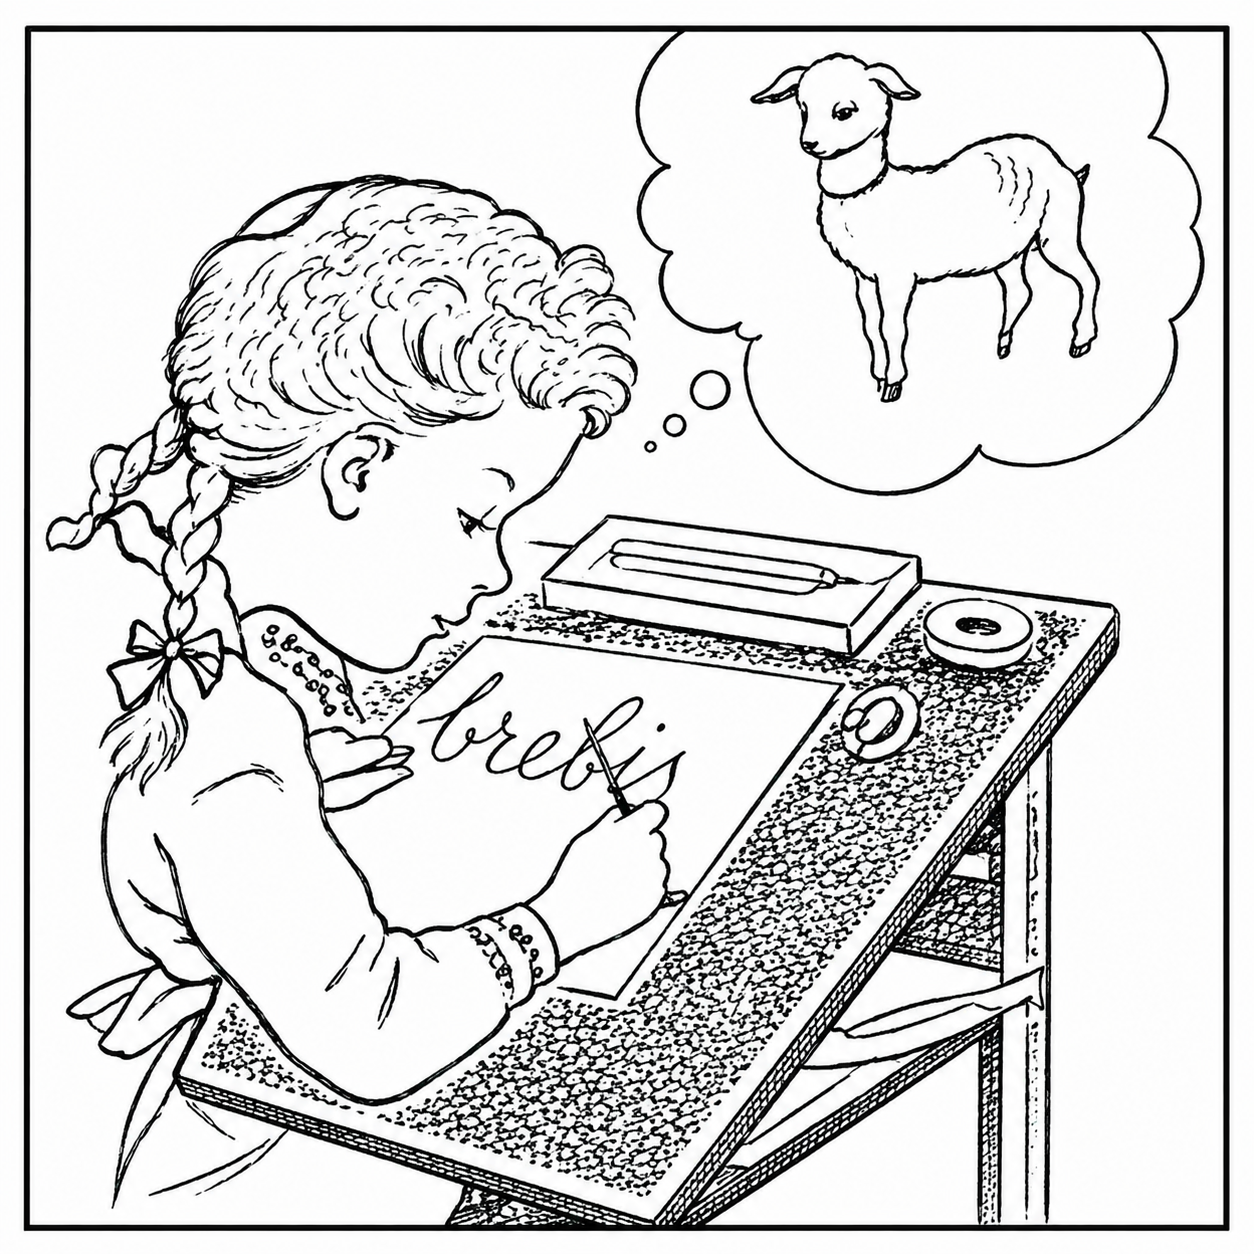
\includegraphics[width=\linewidth]{imgs/111}
\end{wrapfigure}

\textbf{Armandou}, je partage souvent son banc et il est heureux près de
moi. Je travaille à traduire et à franciser son patois. Tout
doucement nous passons des voyelles ... ; aux syllabes et enfin
aux mots qui, parfois, le font rire aux nez dessinons souvent.
J’ai oublié l’infaillible méthode globale de l’Ecole Normale. Mais
Armandou est très appliqué et n’a pas de difficulté en calcul.
Toujours est-il qu’en fin d’année il sait écrire et à peu près lire et
compter. Neuf mois, ce fut long, mais je crois profitable. Qu’est
devenu Armandou ? Il quitta, peu après, le hameau avec sa
famille.
\end{minipage}

\textbf{Le Temple - Ecole. Un peu d’histoire}

Aux lecteurs étonnés de la situation de ce temple-école à Meyrueis (Les Oubrets) je
crois devoir faire part, à posteriori, de mes réflexions, de mes hypothèses aussi, sur
cet état de fait :

Un constat d’abord : sur la rive gauche de la Jonte de nombreux ruisseaux, la Brèze
(le plus important) : le Bétuzon, le Jontanels et bien d’autres rus, s’enfoncent
profondément dans le massif de l’Aigoual. Les petits hameaux, plus ou moins
importants, étaient et sont encore pour ce qu’il en reste, acquis à la Réforme. Ne peut-
on supposer alors, que, très difficiles d’accès, ils ne soient devenus des refuges pour
échapper à la Contre-Réforme du début du 18\ieme{} siècle, à laquelle fut soumise
Meyrueis et la rive droite de la Jonte vers le Causse Méjean ?

Ce petit temple apparaît alors comme une œuvre collective des Huguenots dans le
hameau le plus important « Les Oubrets », facilement accessible aux fidèles par les
sentiers de montagne et apparaît, peut-être, l’idée adjointe de l’utiliser aussi
comme maison d’école pour les enfants d’une communauté protestante
traditionnellement laïque.

D’où une situation confuse et mal définie : temple propriété privée, mais aussi école
publique à fonds publics qui a perduré jusqu’en 1941.
J’ai appris par les habitants du village qu’au moins trois de mes prédécesseurs aux
Oubrets étaient d’origine réformée : Melle B de Rousse, Melle Carrière de Ste Croix-
Vallée- Française et une institutrice de Massevaques dont j’ai oublié le nom.

Et alors... moi-même le seul élève-maître d’origine protestante, d’une promotion de
dix sortants, ne fus-je pas considéré comme le plus à même de s’accommoder de cette
situation particulière ? je me suis souvent posé la question, à laquelle j’éviterai de
répondre : simple hypothèse qui n’engage que moi-même.

% ------------------------------------------------------------
% Page 105
% ------------------------------------------------------------

L’Ecole fut fermée en 1940-41. Elle fut réouverte en 1942. Mon successeur, M. B. de
Villefort, utilisa la salle de classe mais son épouse ne souhaita pas occuper la sacristie
et le ménage trouva à se loger dans le hameau.
Pour clore ce chapitre, ennuyeux pour d’autres que moi-même j’indique que le
pasteur et sa jeune femme sont bien venus célébrer le culte en 1938 devant une salle
comble.

J’ajoute que l’école fut définitivement fermée en 1944, que le temple fut désaffecté et
acquis, peu après par les frères Rousset qui, après aménagement, en firent leur maison
d’habitation où je leur rendis visite quelques années plus tard.

Le hameau, dès la fin de la guerre, a connu le destin de tous les villages de
campagne ; les Rousset, eux-mêmes se retirèrent à Pourcarès, hameau moins éloigné
de Meyrueis. La maison forestière de Vaballe fut abandonnée mais quelques jolis
chalets de pêcheurs, occupés à la belle saison, se sont dressés au bord de la route qui
domine la jolie rivière à truites qu’est restée la Brèze.

Je suis bien conscient que mes réflexions et hypothèses m’ont emmené bien loin de
mon projet initial : « Vous faire part des problèmes auxquels nous fûmes confrontés,
ma femme et moi durant notre séjour de 9 mois dans notre « temple-école ». Mais aux
souvenirs qu’on voudrait évoquer s’attachent d’autres souvenirs qu’il est difficile de
dissocier et d’éluder ;

\begin{center}
\textbf{La vie quotidienne : problèmes à résoudre :}
\end{center}

\textbf{Le ravitaillement}

Facilement résolu. Un épicier ambulant « le Caïffa » livrait à domicile, tous les
samedis, tout ce qui était essentiel pour la semaine : pain, vin, légumes verts ou secs,
fruits et tout un arsenal de conserves sans oublier les bidons de pétrole dont nous
faisions une grande consommation durant les mois d’hiver.
Pour d’autres petits achats je descendais quand même assez souvent à Meyrueis et, au
moins toutes les fins de mois, pour retirer à la perception mes 1030 f. d’émoluments
mensuels. Mon épouse, peu douée pour le vélo, descendit à pied au chef-lieu mais
revint épuisée par les 25 km de l’aller et retour. Elle ne renouvela pas l’expérience et
ne connut de Meyrueis que nos passages rapides lors de nos départs et retours de
vacances.

\textbf{Le chauffage}

A neuf cent mètres et plus d’altitude nous subissions un froid intense dans notre petit
deux pièces et d’autant plus que cuisine et chambrette étaient dépourvues de volets
protecteurs. Mon vieux pardessus d’Ecole Normale étendu devant « le fenestrou »
pour nous protéger de la lumière, était souvent le matin, selon l’expression consacrée,
aussi « raide que la justice ».

% ------------------------------------------------------------
% Page 106
% ------------------------------------------------------------

\begin{wrapfigure}{l}{0.35\textwidth}
    \centering
    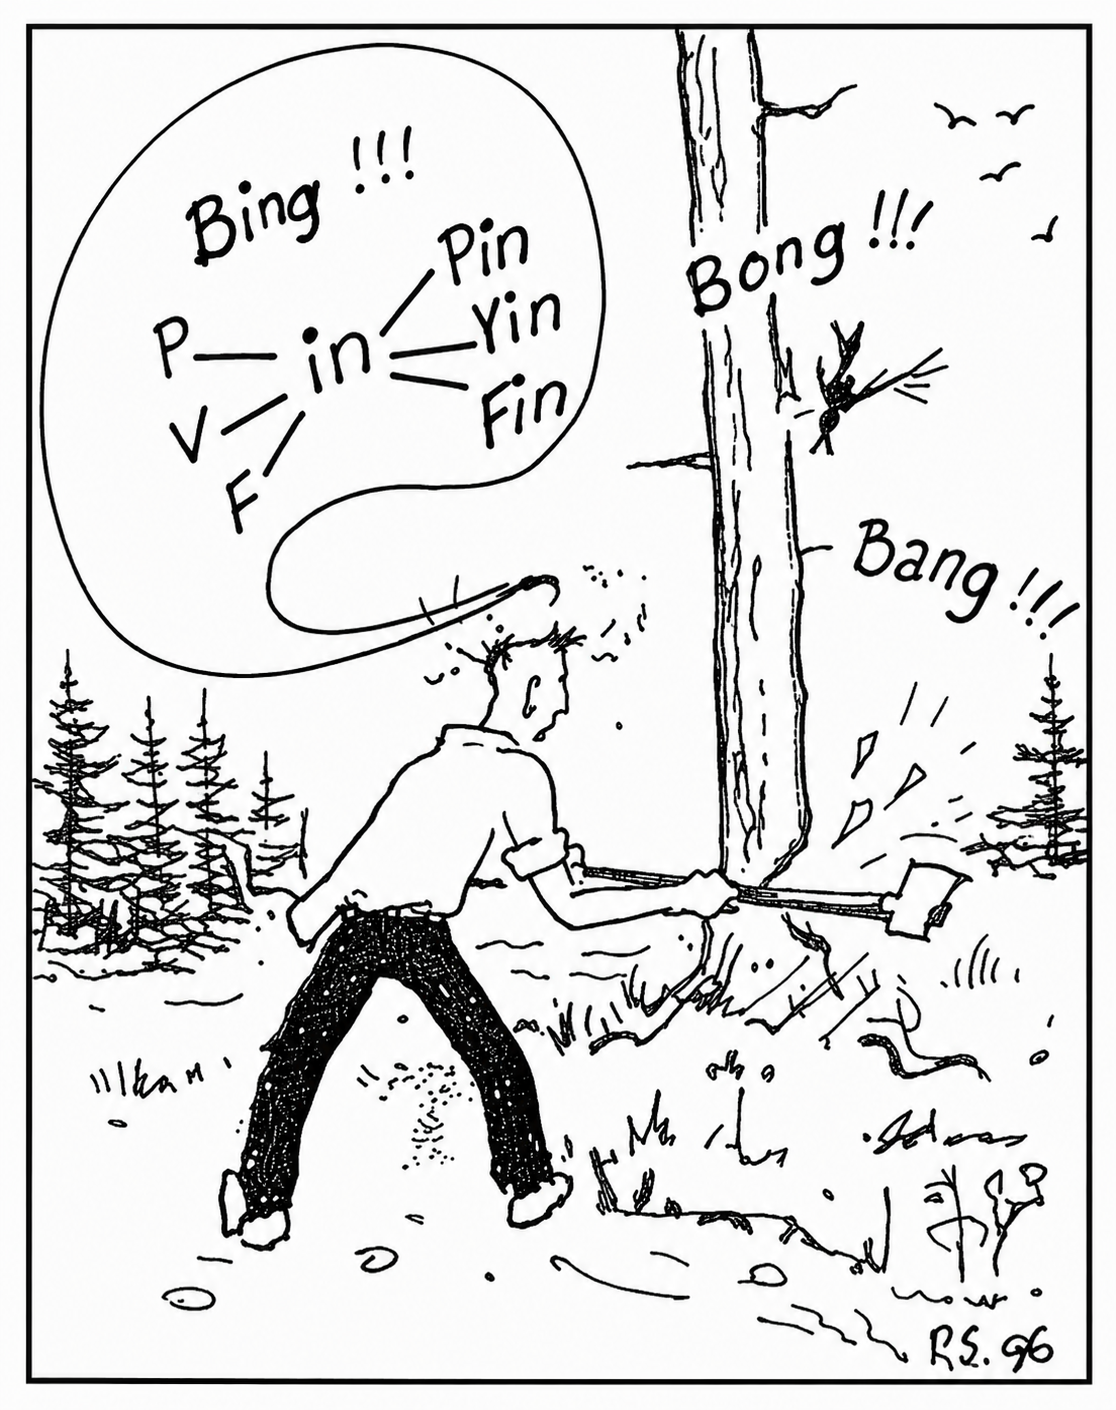
\includegraphics[width=\linewidth]{imgs/113}
\end{wrapfigure}

Le « voyage de bois » non scié, fourni par
M. le Maire ne résista pas longtemps aux
besoins confondus du poêle de l’école et
de notre cuisinière.
Par nécessité je devins alors instituteur
bûcheron et, dès la fin novembre je
passais le plus clair de mes jeudis et
dimanches dans la forêt domaniale qui
s’étendait jusqu’à la Serreyrède.
Moyennant une redevance de 6 F versés
au garde-forestier de Valbelle, je pouvais
couper parmi les arbres morts,
complètement ébranchés, tout ce qui était
à ma convenance. J’avais une bonne
hache et assez d’expérience pour orienter
la chute des troncs en tous points
semblables à de longs poteaux
télégraphiques.

Tout au long de la route forestière, j’étalais donc l’équivalent de deux gros « voyage »
que le père de Martin, fort gentiment et gratuitement : me ramena jusqu’à l’école.
Commença alors le long et combien pénible travail de sciage. La « tronçonneuse »
d’alors, donc la scie à mains, même bien affûtée, graissée, ne fonctionnait « qu’à
l’huile de coude ».

Fendre les rondins obtenus en quatre bûches n’était alors qu’un jeu. Marin, qui avait
la responsabilité du poêle et du bûcher, s’activait pour dresser et équilibrer les piles
de bois devant la grande porte, selon les conseils de M. l’Inspecteur, pour éviter les
courants d’air.

\textbf{L’environnement}

L’école ne disposait pas de WC. Il n’en restait pas moins que, comme tous les
mortels, il fallait satisfaire à certains besoins « biologiques ». Au cours de
promenades matinales j’acquis une connaissance précise de l’environnement et des
possibilités d’en tirer avantage.

La cuisinière allumée, la tasse de café avalée, par tous les temps, plus ou moins
chaudement vêtu, je partais.... promener. La chance voulut que, dès mes premières
sorties, des grives (draines), des merles s’envolent de deux sorbiers au bord d’un ru.
Je ne fus pas long à comprendre. Dès lors mon fusil, ramené des Grottes lors de ma
première visite, devint le compagnon idéal. Mes chasses, bien sûr, n’intéressent
personne mais je les cite seulement pour dire que de novembre à fin mars il y eut
toujours des grives à la maison. Les jours de grive, de brouillard ou de neige
poudreuse les litornes s’abattaient par centaines sur les genévriers découverts un peu
plus haut. Une salve meurtrière, je ramassais les victimes et rentrais en courant,
pressé de glisser mes pieds sur la plaque chaude du four de la cuisinière. Ma femme
s’occupait du reste. Elle évoqua souvent les souvenirs gourmands de ses préparations
en salmis, à la tartine.

% ------------------------------------------------------------
% Page 107
% ------------------------------------------------------------

Si j’ajoute à cela que les jours de beau soleil il suffisait de sauter la rivière, de rester
immobile à la lisière d’un bosquet de sapins et d’attendre le léger grignotement qui
révélait l’écureuil promis à un délicieux petit civet… Tout cela pour dire que la
viande que n’apportait pas « le Caïffa » ne nous manquait nullement et d’autant plus
que sur les conseils et l’aide de Ricau A. je devins au printemps un pêcheur, disons
passable, mais largement suffisant.

Tous les jours vers dix heures, nous surveillions l’arrivée du facteur, poussant sa
bicyclette, il distribuait le courrier, visitait la boite aux lettres avant d’entrer chez
nous où le café l’attendait. Il déposait à la maison le quotidien de Rousset « La
Dépêche de Toulouse » qu’ils ne consultaient que le soir. Nous avions toute la
journée pour lire et éplucher au jour le jour l’actualité de cette année 1939 fertile en
événements qui furent souvent déterminants pour les années qui suivirent. Le jeune
facteur nous proposait tous les jours ses services pour tout ce dont nous pourrions
avoir besoin. Nous n’abusions pas parce qu’il refusait toujours le prix du morceau de
viande s’estimant lui-même redevable de quelques grives ou plus tard de quelques
truites que nous lui offrions occasionnellement.

\begin{center}
\textbf{Les Habitants des Oubrets}
\end{center}

L’environnement c’était aussi le hameau et ses habitants mais là, je laisse tomber la
plume, car c’est un paragraphe que je devrais consacrer à chacune des familles ;
disons seulement que toutes étaient toujours prêtes à nous être agréables. Ainsi la
brave dame s’arrêtant devant notre porte : « Il fait très froid aujourd’hui, donnez-moi
donc votre petite lessive, je la rincerai avec la mienne ». Il est vrai que ma jeune
épouse avait conquis tout le monde car elle avait su tout de suite visiter mais aussi
recevoir. On venait souvent la voir pour des raisons les plus diverses ( relever un
modèle de tricot, par exemple, ou, tout simplement bavarder).

Bien sûr nous étions invités à toutes les agapes et les festins hivernaux et le
lendemain figurait encore sur notre table la petite « padelade » traditionnelle
(boudins, tranches de rôti, et bout de saucisse).

Et puis encore de temps à autre : « Voici un verre de pâté ou une assiette de cervelas,
j’ai eu peut-être la main un peu lourde pour le sel… on le mangera comme ça
etc..etc.. Nous étions un peu gênés par tant de générosité, nous qui n’avions à
offrir que quelques tasses de café.

Je ne résiste pas à l’envie d’écrire quelques mots sur deux personnes fort différentes
mais faisant preuve à mon égard d’une grande confiance :

\textbf{« POLICE ».} On ne l’appelait qu’ainsi, était un vieux célibataire, un grand-oncle de
Mme. Argeliers --mon ancienne restauratrice du mois d’octobre-- qui l’hébergeait. Il
venait de temps à autre à la maison pour se chauffer peut-être, mais aussi pour me
répéter : » Vous savez, je ne suis pas « un sans le sou », et d’étaler sur la table et de
compter devant moi un pécule de 1450 F. (1939), visiblement heureux devant tant
d’argent qu’il repliait soigneusement avant d’introduire le précieux portefeuille dans
une poche intérieure méticuleusement épinglée.

% ------------------------------------------------------------
% Page 108
% ------------------------------------------------------------

\textbf{« ARGELIERS »} le mari de Mme. Argeliers, la casquette de travers, long « comme
un jour sans pain » m’avait pris en amitié. C’était un piégeur professionnel de fouines
et de martres dont les peaux se négociaient à Millau, au prix fort de 6 à 800F. de
l’époque. Il me proposa de l’accompagner ne voyant pas en moi un « concurrent
possible ! ». Je le suivis dans des endroits impossibles dans le silence de ses pas
feutrés ; sans parole, il me montrait du doigt l’emplacement où se trouvaient les
pièges, mais je ne distinguais rien ; lui, à d’infinis détails, il voyait et savait. Ce jour-
là nous revînmes bredouilles mais il me confia que les mois d’hiver il gagnait pour
toute l’année.

Les beaux jours revinrent ; durant le mois de mai on installa l’électricité et je fus
surpris d’apprendre que la maison d’école ne figurait pas sur le projet. Je crus donc,
par devoir vis-à-vis de mon possible successeur, d’alerter encore une fois M. le
Maire... La réponse fut brève : « La Mairie de Meyrueis n’est en rien concernée. » Je
partis en claquant la porte.

\begin{center}
\textbf{Juin-juillet : Fin de l’année scolaire}
\end{center}

\textbf{Juin :}

Nous faisions de longues promenades dans les forêts domaniales, scrutant les fossés,
espérant découvrir morilles ou quelques cèpes, mais ce printemps-là, trop sec, n’était
pas favorable. Un jour, longeant un sentier remontant la rivière, nous fûmes étonnés
d’atteindre si vite le col de la Serreyrède et là, signalé à 2km, le village de l’Espérou
qui avait déjà une vocation touristique. Sur notre lancée nous arrivâmes au village.
C’était le jour de la fête votive ; nous y participâmes quelques heures avant de
reprendre le chemin du retour qui fut, par les pentes, très rapide, réalisant que
pédestrement nous étions plus proches de l’Espérou que de Meyrueis.

\textbf{Juillet :}

Notre départ était proche. Comment pouvions-nous remercier les gens de leur bon
accueil, de leur aide prodiguée gratuitement en bien des circonstances ?
L’idée nous vint de réunir au temple nos amis, c’est à dire tout le monde non pas pour
y entendre « la bonne parole », mais pour partager avec nous de modestes
« festivités ». Encore une fois nous déplaçames tables et bancs, on nous prêta tables et
chaises, vaisselle... car tout le monde voulait participer, le « Caïffa » nous livra, sur
commande, tout ce qui était nécessaire pour organiser un « buffet » honorable. Tout le
monde répondit à notre invitation : la soirée se prolongea fort tard et nous fûmes
heureux.

% ------------------------------------------------------------
% Page 109
% ------------------------------------------------------------

Ainsi se termina notre séjour aux Oubrets. Comment conclure ? Disons que tout n’y
fut pas rose, surtout les premiers mois ; mais les bons souvenirs (et ils sont
nombreux) estompent les mauvais, les liens de l’amitié résistent au temps. Ainsi
Adrien Rousset, de retour de la Foire de Sainte-Croix-Vallée-Française, fit un crochet
par le mas Rotger pour nous dire bonjour, et c’est la famille Argeliers qui nous rendit
visite à Bassurels.

J’ai amené plusieurs fois ma famille aux Oubrets pour constater, hélas, la désolation
d’un hameau qui fut prospère, celui de nos vingt ans.

\begin{flushright}
Nîmes le 24 Février 1996
\end{flushright}

\begin{flushright}
André BAZALGETTE
\end{flushright}

\begin{figure}[ht]
    \centering
    % À remplacer par le fichier image correspondant
    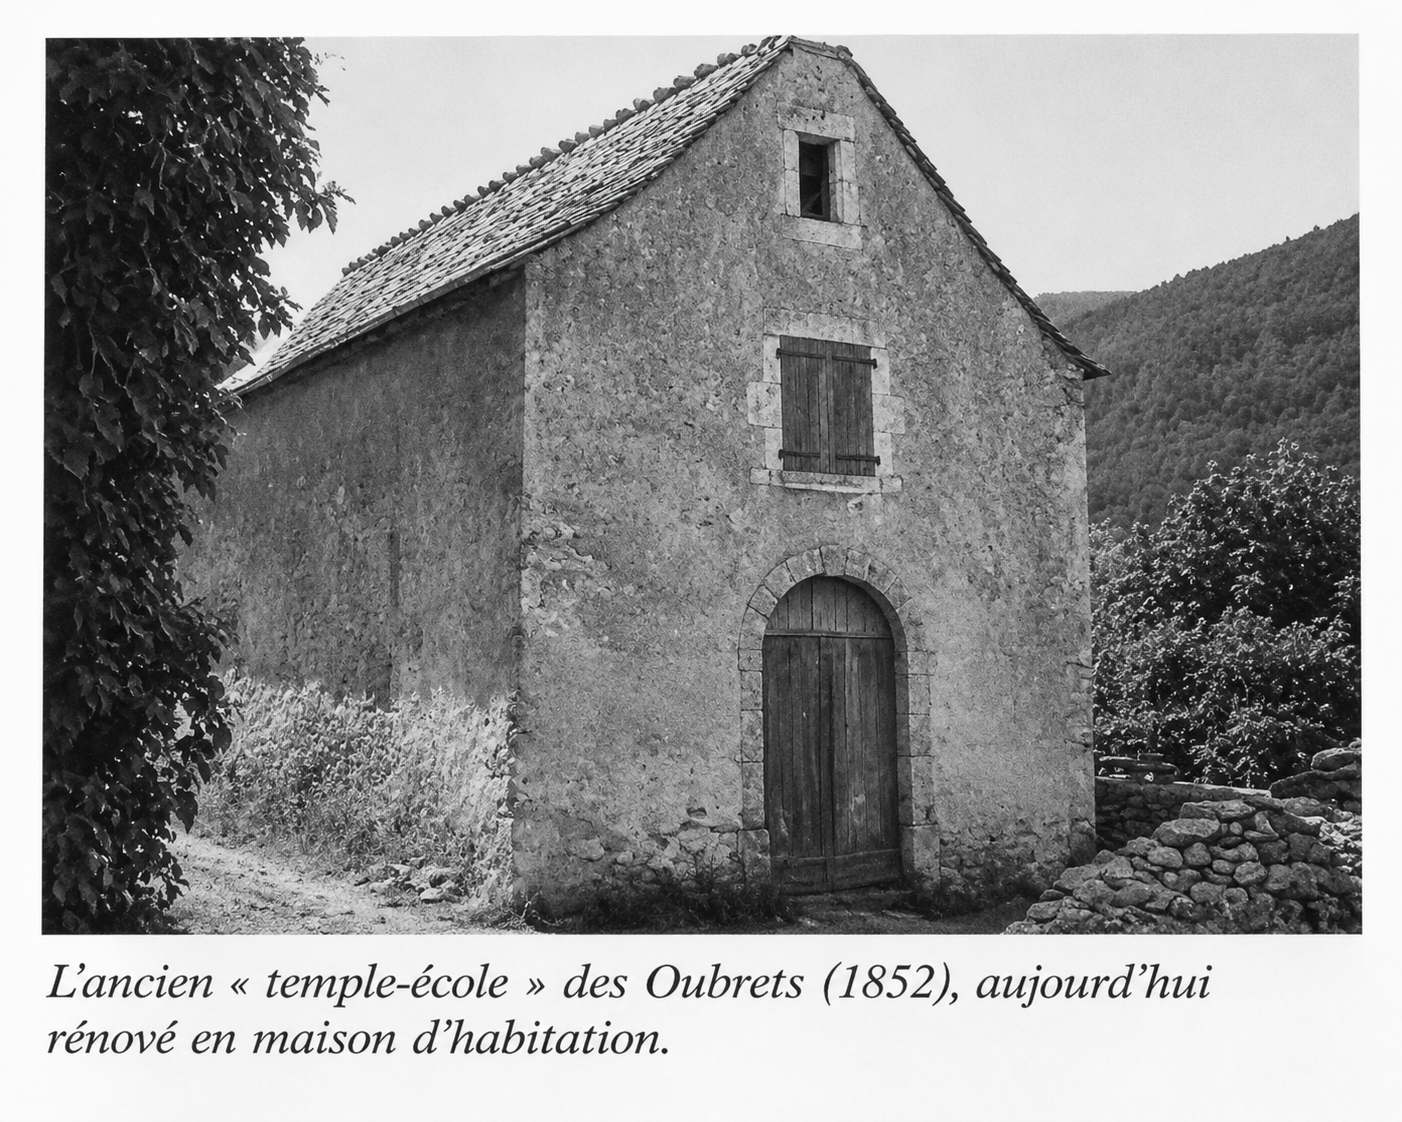
\includegraphics[width=0.38\textwidth]{imgs/116}
    
    \caption{\textit{L’ancien « temple-école » des Oubrets (1852), aujourd’hui
    rénové en maison d’habitation.}}
\end{figure}
